\documentclass[12pt, letterpaper, oneside]{memoir}
\tolerance=1000 % sets whitespace tolerance level (adjusts hyphenation)

% *************** Document style definitions ***************

% ******************************************************************
% This file defines the document design.
% Usually it is not necessary to edit this file, but you can change
% the design if you want.
% ******************************************************************

% The origin of this file is not clear.  Here is one copy:
% https://subversion.cs.uu.nl/repos/staff.doaitse.wxFlashkell/MasterThesis/style_old.tex
% Emerson Murphy-Hill (emerson@cs.pdx.edu) has modified it.
% Jarrett Keifer (jkeifer@pdx.edu) has also modified it greatly. It is now using AAG format for the references, suitable for all geography theses.


%************************* NOTES ON FORMATTING *************************

%Spacing:
%  Cannot use the setspace package with memoir class. However, memoir has its own spacing commands, and they are exactly the same, except use camel-casing:
%    \begin{Spacing}{1.5} or \DoubleSpacing or \OnehalfSpacing or \SingleSpacing


% *************** Load packages ***************
% *************** Colors ***************
\usepackage[usenames, dvipsnames]{color}
%\definecolor{bg}{rgb}{0.95,0.95,0.95} 


% **************** Syntax Highlighting ******************
\usepackage{minted} %for code snippets; use \begin{minted}[mathescape, linenos, etc]{python}
\usemintedstyle{tango}


% ****************** For Figures and Graphics *******************
\usepackage{graphicx}
\usepackage[justification=centering, labelfont=bf, small, compatibility=true]{caption} %caption package with centering, and can be 10pts, per thesis guidelines
\usepackage{subcaption} %allows subfigure captions
\captionsetup[sub]{font=footnotesize} %The subcaption settings
\captionsetup{compatibility=false} %To make caption package work
%\usepackage{cleveref} %Use \cref to add prefix to refs (i.e. Fig., Table, etc.)
%\usepackage{flafter} %Don't place floats until after refs

%To define \captionabove command for tables
\makeatletter
\newcommand{\captionabove}[2][]{%
    \vskip-\abovecaptionskip
    \vskip+\belowcaptionskip
    \ifx\@nnil#1\@nnil
        \caption{#2}%
    \else
        \caption[#1]{#2}%
    \fi
    \vskip+\abovecaptionskip
    \vskip-\belowcaptionskip
}


% ************** ALL OTHERS **************

\usepackage{varioref} 
\usepackage{times}
\usepackage{comment}
\usepackage{amssymb}
\usepackage{amsmath}
\usepackage{ifthen}
\usepackage{multirow}
\usepackage{xspace}
\usepackage{url}
\urlstyle{sf}
\usepackage{makeidx}
\usepackage{needspace}
\usepackage{tabularx}
\usepackage{colortbl}
\usepackage{enumitem}
\usepackage{afterpage}
\usepackage{longtable}
\usepackage{lscape}
\usepackage{ulem}
\usepackage{epsfig}
\usepackage{amsthm}
\usepackage{booktabs}
\usepackage{stmaryrd}
\usepackage[figuresright]{rotating}
\usepackage{xltxtra} %Xeletex Package
\usepackage{fontspec} %Font package
\usepackage{xunicode} %Xeletex

\normalem %normal emphasis for package ulem
\vrefwarning %warnings, not errors, for vrefs for varioref package

%TODO MOVE ALL GROUPS OF SETTINGS (I.E. TABLES & FIGURES, DOCUMENT LAYOUT, ETC. TO NEW TEX FILES INSIDE A SETTINGS FOLDER]


% *************** Enable index generation ***************
\makeindex


% **************** Language/Localization ***************
\usepackage[australian, spanish, american]{babel} %datetime incompatible with polyglossia
%\usepackage{polyglossia}
%\setdefaultlanguage[variant=american]{english}
%\setotherlanguage{spanish}


% *************** Set Date Format ***************
\usepackage[nodayofweek]{datetime}
%\setdefaultdate{\dateaustralian} %gets dates of dd month yyyy without ordinal or comma


% ********* Reference Settings **********
\input{bibsettings.tex}


% *************** Set Fonts ***************
\defaultfontfeatures{Ligatures=TeX}
\setromanfont[Mapping=tex-text]{Baskerville}
\setsansfont[Mapping=tex-text]{Myriad Pro}
\newfontfamily\titleFont[Ligatures=TeX]{Myriad Pro}
\setmonofont{DejaVu Sans Mono}


% *************** Page layout ***************
%\settypeblocksize{*}{32pc}{1.618}

\setlrmarginsandblock{1.5in}{1.0in}{*}  % Left and right margins
\setulmarginsandblock{1.5in}{1.0in}{*}  % Top and bottom margins
\checkandfixthelayout

\setheadfoot{\onelineskip}{2\onelineskip}
%\setheaderspaces{*}{2\onelineskip}{*}

\def\baselinestretch{2}  % double space for PSU

\checkandfixthelayout


% *************** Chapter and section style ***************
\makechapterstyle{mychapterstyle}{%
    \renewcommand{\chapnamefont}{\normalfont\sffamily\bfseries\large}%
    \renewcommand{\chapnumfont}{\normalfont\sffamily\bfseries\large}%
    \renewcommand{\chaptitlefont}{\normalfont\sffamily\bfseries\LARGE}%
    \renewcommand{\printchaptertitle}[1]{%
        \chaptitlefont{##1}
        }%
    \renewcommand{\printchapternum}{%
        \chapnumfont\thechapter%
        }%
       
}

\renewcommand*{\cftappendixname}{Appendix\space}

\chapterstyle{mychapterstyle}

\setsecheadstyle{\normalfont\sffamily\bfseries\large}
\setsubsecheadstyle{\normalfont\sffamily\bfseries}
\setsubsubsecheadstyle{\normalfont\sffamily\bfseries}
\setparaheadstyle{\normalfont\sffamily}

\nouppercaseheads  % prevents the headers from being uppercase
\makeevenhead{headings}{\normalfont\sffamily\mdseries\rightmark}{}{\normalfont\sffamily\mdseries\thepage}
\makeoddhead{headings}{\normalfont\sffamily\mdseries\rightmark}{}{\normalfont\sffamily\mdseries\thepage}

\aliaspagestyle{chapter}{empty}%this suppresses numbers on chapters


% *************** Table of contents style ***************
\settocdepth{subsubsection}

\setsecnumdepth{subsubsection}
\maxsecnumdepth{subsubsection}
\settocdepth{subsubsection}
\maxtocdepth{subsubsection}


% ********** Commands for epigraphs **********
\setlength{\epigraphwidth}{0.57\textwidth}
\setlength{\epigraphrule}{0pt}
\setlength{\beforeepigraphskip}{1\baselineskip}
\setlength{\afterepigraphskip}{2\baselineskip}

\newcommand{\epitext}{\sffamily\itshape}
\newcommand{\epiauthor}{\sffamily\scshape ---~}
\newcommand{\epititle}{\sffamily\itshape}
\newcommand{\epidate}{\sffamily\scshape}
\newcommand{\episkip}{\medskip}

\newcommand{\myepigraph}[4]{%
	\epigraph{\epitext #1\episkip}{\epiauthor #2\\\epititle #3 \epidate(#4)}\noindent}
	
	
% **************** Blank Page Commmand ***************
\usepackage{afterpage}
\newcommand\blankpage{%
    \null
    \thispagestyle{empty}%
    %\addtocounter{page}{-1}%
    \newpage}
    

% *************** DRAFT OPTIONS ****************
\usepackage{ifdraft}
%\ifdraft{<draft case>}{<final case>}
%\ifoptiondraft {⟨option draft given⟩} {⟨option draft not given⟩}
%\ifoptionfinal {⟨option final given⟩} {⟨option final not given⟩}

% *************** Enable hyperlinks in PDF documents ***************
\ifpdf
    \pdfcompresslevel=9
        \usepackage[plainpages=false,pdfpagelabels,bookmarksnumbered,%
        colorlinks=true,%
        linkcolor=sepia,%
        citecolor=sepia,%
        filecolor=maroon,%
        %pagecolor=red,%
        urlcolor=sepia,%
        pdftex,%
        unicode]{hyperref} 
    \pdfimageresolution=600
    \usepackage{thumbpdf} 
\else
    \usepackage{hyperref}
\fi
\usepackage[all]{hypcap}  % fixes problem when  you click on a link and go to caption, not figure or table itself

\usepackage{memhfixc}


% *************** End of document style definition ***************  % Contains all the packages, commands, and formatting settings

\newcommand{\refacName}[1]{\textsc{#1}}
\newcommand{\needlines}[1]{\Needspace{#1\baselineskip}}
\newcommand{\thesisTitle}{Phenological classification of crops in Northwest Argentina using 250-meter MODIS imagery}
\newcommand{\thesisAuthor}{Jarrett A. Keifer}
\newcommand{\thesisDegree}{Master of Art}
\newcommand{\thesisDept}{Geography}
\newcommand{\thesisDate}{June 11, 2014}
\newcommand{\thesisAdvisor}{Jiunn-Der Duh}
\newcommand{\thesisCommitteeOne}{David Banis}
\newcommand{\thesisCommitteeTwo}{Leopoldo Rodriguez}
%\newcommand{\thesisCommitteeThree}{committee3}
\newcommand\thesisAbstract{%
Subtropical deforestation in Latin America is thought to be driven by demand for agricultural land, particularly to grow soybeans. However, existing remote sensing methods that can differentiate crop types to verify this hypothesis require high spatial or spectral resolution data, or extensive ground truth information to develop training sites, none of which are freely available for much of the world. Here, I propose a new method of crop classification using multi-temporal MODIS vegetation indices as a base image from which to extract crops using their phenologies. I test and refine this method in Kansas, USA using the USDA crop data layer as reference. I then test the applicability of the method to other regions of the world by applying it to data from Pellegrini, Santiago Del Estero, Argentina. The study is to examine if using phenological profiles in image classification is a viable method to verify the initial hypothesis that soybeans are driving deforestation in subtropical South America.
}

\newcommand\chapterWithSubtitle[2]{\chapter[#1]{#1: #2}}

\makeatletter
\def\url@leostyle{%
  \@ifundefined{selectfont}{\def\UrlFont{\sf}}{\def\UrlFont{\small\sffamily}}}
\makeatother
\urlstyle{leo}

\newcommand\gc{\rowcolor[rgb]{0.93,0.93,0.93}}

\renewcommand{\texttt}[1]{{\small\ttfamily #1}}
%\renewcommand{\textsf}[1]{{\small\sffamily #1}} % for some reason, this kills all the refs!


% *************** THE DOCUMENT ***************
\begin{document}


% *************** Front matter ***************
\frontmatter
\pagenumbering{Roman} 
\pagestyle{empty} 



\long\def\signature#1#2{
\begin{flushright}
\begin{minipage}{200mm}
\begin{flushleft}
\vspace{.3in}
#1\\
\hbox to 135mm{\hfil\shortstack[l]{\vrule width 60mm height 0.4pt\\#2}}
\end{flushleft}
\end{minipage}
\end{flushright}}

 \begin{center} THESIS APPROVAL \end{center}
        \noindent The abstract and thesis of \thesisAuthor~for 
        the \thesisDegree~in \thesisDept~were presented on \thesisDate,
        and accepted by the thesis committee and the doctoral program.        

    \signature{COMMITTEE APPROVALS:}\thesisAdvisor    
    \signature{\ }\thesisCommitteeOne
    \signature{\ }\thesisCommitteeTwo
    %\signature{\ }{\thesisCommitteeThree\\Representative of the\\Office of Graduate Studies}    
    %\signature{DOCTORAL PROGRAM APPROVAL:}{Wu-chi Feng, Director\\Computer Science Ph.D. Program}

\clearpage



\begin{center}
ABSTRACT
\end{center}
 
\noindent
An abstract of the thesis of \thesisAuthor~for the \thesisDegree~in 
\thesisDept~presented \thesisDate.
     
\vspace{15mm}
     
\begin{hangparas}{20mm}{1}
    Title: \thesisTitle
\end{hangparas}

\vspace{15mm}
\thesisAbstract




\clearpage
    
\begin{center}
	~\\
	~\\
	~\\
    \MakeUppercase {\thesisTitle} 
\end{center}

\begin{center}
    by\\
    \vspace{2mm}
    \MakeUppercase{\thesisAuthor}
\end{center}

\vfill\vfill

\begin{center}
    A thesis submitted in partial fulfillment of the\\
	\vspace{-2mm} 
    requirements for the degree of
\end{center}

\vfill

\begin{center}
     \MakeUppercase{\thesisDegree}\\
     \vspace{-2mm} 
     in\\
     \vspace{-2mm} 
     \MakeUppercase{\thesisDept}
\end{center}


\vfill

\begin{center}
    Portland State University\\
    \vspace{-2mm} 
    2014
\end{center}

\cleardoublepage    

\begin{center}
    \vspace*{2.5 in}
    \copyright~2014 \thesisAuthor
\end{center}

\cleardoublepage

\pagenumbering{roman}

\vspace*{\fill}
{\hfill\sffamily\itshape Something fancy.}


\rmfamily
\normalfont


\chapter*{Acknowledgements}
\addcontentsline{toc}{chapter}{Acknowledgements}

\pagestyle{headings}

Something goes here.

\clearpage
 


\tableofcontents



\clearpage
\listoftables

\clearpage
\listoffigures





% *************** Main matter ***************

\mainmatter
\chapter{Introduction}
\label{intro}

Deforestation has long been a concern throughout tropical South America. However, this process of land use/land cover (LULC) change from forest to other uses has been increasingly recognized in subtropical South America as a significant source of environmental degradation. Understanding the complex dynamics of subtropical deforestation is crucial given the prominent role of forests in debates about climate change, conservation, and the protection of endangered species \autocites{geist2002proximate}{zak2004do-subtropical}{bonnie2000counting}{houghton1994the-worldwide}{sala2000global}.

Currently, many perceive growing demand for agricultural land---particularly land for soybeans---to be one of the greatest pressures on South American subtropical forests \autocites{pengue2005transgenic}{grau2005agriculture}{altieri2006gm-soybean:}. Remote sensing has given researchers a tool to classify land cover and measure deforestation. However, existing multi-spectral and multi-temporal image classification techniques require extensive ground truth information for the accurate classification of common crop types using widely-available remotely-sensed data. Therefore, getting a complete picture of the dynamics of deforestation, including an understanding of agricultural pressures on forests, requires rarely-available high spatial or high spectral resolution data \autocite{senay2000using} or expensive field time gathering training site data. The development of a tool that can efficiently and effectively extract crop types using widely-available imagery would be of value in investigations of LULC change in areas under rapid agricultural expansion.

The primary goal of this thesis is to develop and test a phenological classification toolset that can identify and extract crop types from a multi-date vegetation index sequence assembled using free and publicly-accessible data from the National Aeronautics and Space Administration’s (NASA) Moderate Resolution Imaging Spectroradiometer (MODIS) sensor. The toolset was tested using the U.S. Department of Agriculture's (USDA) Cropland Data Layer (CDL) from a test field in Kansas, USA. The CDL data provided delineation and crop identification of agricultural fields in the study area. Overlaid on the MODIS data, the CDL crop boundaries allowed the extraction of reference phenological signatures for various summer crops. Using the Kansas-derived reference signatures, imagery of the 2014 summer growing season in the Department of Pellegrini, Santiago del Estero, Argentina was then classified with the toolset. I further preformed a classification accuracy assessment to examine the toolset's applicability in subtropical South America.

The body of this thesis is broken into seven chapters. The \hyperref[intro]{first chapter} gives an overview and an introduction of the research. The \hyperref[background]{second chapter} provides background information on deforestation and soybean cultivation in Argentina. \hyperref[studyareas]{The third} introduces the two study areas where the processing methods, presented in \cref{methods}, are applied. \Cref{results} reviews the results of said methods, and \cref{discussion} is a discussion of their significance. \cref{conclusion} closes the thesis with some concluding remarks.

An additional five appendices contain supporting information. \Cref{appendix:fieldwork} is a reflection of my time in Argentina doing the fieldwork for this project. \Cref{appendix:tools} documents the toolset created to implement the processing methods of \cref{methods} and the development process. All the initial testing of the tools is reviewed in \cref{appendix:testing}. \Cref{appendix:future} contains a collection of ideas for future testing and research. Lastly, \cref{appendix:cdl} is a brief note about the CDL dataset.
\chapter{Background}
\section{Deforestation and the \textit{Ley de Bosques} (Forest Act) in Argentina}

The conversion of forestland to other uses has seriously impacted Argentina’s forests. In 1915 it was remarked that 30 percent of the country had forest cover, but in 2001 only 10 percent remained forested \autocite{secretaria-de-d2001primer}. Over the period 1998 to 2002, Argentina lost over 940,000 hectares of forest cover \autocite{secretaria-de-a2007informe}. The high rate of deforestation concerned policymakers, and Law 26.331, or the \textit{Ley de Bosques} (Forest Act), was voted into law in 2007 in an effort to preserve remaining native forests. Areas of native forest are defined to be those with forest cover of at least 20 percent native species, and that have trees of a minimum of 7 meters high. The law designates red, yellow, and green areas, each with different restrictions on clearing and use. Red is assigned to areas of “high conservation value,” yellow is for areas that must be managed sustainably, and green allows “partial or total use” \autocite[25]{gulezian2009environmental}. Each provincial government was responsible for determining how to classify their native forest area, and each enacted the \textit{Ley de Bosques} regulations under the \textit{Ordenamiento Territorial de los Bosques Nativos} (Land Management Order for Native Forests, OTBN).

As a part of Law 26.331, ongoing land cover studies are done to examine the effectiveness of the legislation. Between 2006 and the passing of the law, 573,296 hectares of native forest cover were lost. From the passing of the law in 2007 and the classification of the OTBN areas in 2009, a further 473,001 hectares were deforested. From the enacting of the OTBN (in 2009) and 2011, some 459,108 hectares were found to have been lost \autocite{secreteria-de-a2012monitoreo}. The continued deforestation suggests that, in the context of the native forest areas, the \textit{Ley de Bosques} may have had a small effect in reducing deforestation, but overall levels still remain quite high. Consequently, some have begun to question the effectiveness of the law at slowing cutting \autocites{valpreda2012the-protection}{greenpeace-arge2013ley-de-bosques:}. Clearly, a better understanding of the driving forces of deforestation in Argentina needs to be developed.

\section{Soy and its effects}

The increase of soybean in Argentina has occurred at a rapid pace throughout the last two decades, making it the third largest producer of soy in the world \autocite{us-foreign-agri2013world}. Necessarily, as soy production rises, so does its spatial extent and the intensity of cultivation methods. Currently, almost all of Argentina’s soy production is using genetically modified (GM) varieties, specifically Monsanto’s “Roundup Ready” beans \autocite{greenpeace-inte2005the-expanding}. The highly mechanized and input intensive nature of this crop type calls into question other environmental consequences of soybean cultivation, such as pesticide runoff, glyphosate-resistant weeds, and soil depletion \autocite{pengue2005transgenic}.

A number of studies have addressed soy and deforestation in Northwest Argentina, but only one has used methods capable of mapping crop types in deforested areas \autocite{volante2005analisis}. However, this study by the Argentine \textit{Instituto Nacional de Tecnología Agropecuraia} (National Institute of Agricultural Technology, INTA) does not have well-documented methodology and has not been updated since 2005. Of the remainder, all used remote sensing techniques to classify only LULC and not specific crop types, leaving the effect of soy on LULC as an underlying assumption \autocites{grau2005agriculture}
{grau2008balancing}{grau2005globalization}
{boletta2006assessing}{gasparri2009deforestation}. While the extreme deforestation in Argentina is undeniable---and certainly soy plays a part---its role has not been examined in full, leaving unsubstantiated the perception of soy as the driving force in this process.

The goal of this research is to develop an image classification capable of mapping agricultural crops by type, allowing soy to be explicitly identified on remotely sensed imagery. The accurate and efficient mapping of soy distributions and their changes over time could allow further investigation of the roles of soy in deforestation. The direct and indirect effects soy crops have had on deforestation can thus be understood conceptually and systemically at both regional and local scales, which could lead to the development of more effective policies for land management \autocite{brown2007multitemporal}.

\chapter{Study Areas}
\label{chapter:studyareas}

This study used agricultural areas in Kansas, USA for testing and verification of the phenological classification method and applied the classification method to Pellegrini, Santiago del Estero, Argentina to test its effectiveness in subtropical South America.


\section{Kansas, USA}
\label{chapter:studyareas:kansas}

The state of Kansas is one of the big agricultural producers of the U.S. As one of the plains states, it is relatively flat across much of its extent, making it well suited to large highly-mechanized agro-industrial operations. In 2012, the three most extensive crops in the state were wheat, corn, and soybeans (\autoref{table:kansas}), which are also the most abundant crops in Pellegrini, Argentina. Additionally, Kansas has been the focus of a number of previous studies into the use of MODIS time-series for crop classification \autocites{wardlow2002discriminating}{wardlow2005state-level}{wardlow2007analysis}{wardlow2008large-area}, and has a very detailed and easily-accessible crop cover dataset in the form of the USDA CDL, making it a natural choice for a preliminary study area to test my method.

I have chosen a small 100 MODIS pixel by 100 MODIS pixel study area just northwest of Wichita, Kansas, which includes the communities of Valley Center, Sedgwick, and Halstead running roughly in a line from the southeast corner to the northwest corner (\autoref{fig:KSstudysite}. This is the area where I did testing and verification of the method (see \autoref{appendix:testing} for a full overview of the Kansas testing), and where I extracted the crop reference signatures used for the Argentina classification. The typical planting dates for a variety of crops in this region are shown in \autoref{table:KSplantingdates}. This specific study site was chosen due to the good mix of land covers including, but not limited to, corn, soy, sorghum, winter wheat, winter wheat and soy double crop, urban development, grassland, and forest in the CDL reference.


\begin{sstable}
  \centering
  \caption[Most extensive crops in Kansas, 2012.]{Most extensive crops in Kansas, 2012\\~\autocite[adapted from][]{usda2013kansascrops}.}
  \label{table:kansas}
  \begin{tabu}{lcc}
    \toprule
    \textbf{Crop} & \textbf{Acreage (1,000 acres)} & \textbf{Production (1,000 units)} \\
    \midrule
    Wheat & 9,100 & 382,200 \\
    Corn & 3,950 & 379,200 \\
    Soy & 3,810 & 83,820 \\
    All Hay & 2,750 & 4,340 \\
    All Forage & 2,750 & 4,545 \\
    Sorghum & 2,100 & 81,900 \\      
    \bottomrule
  \end{tabu}
\end{sstable}

\begin{ssfigure}
  \centering
  \includegraphics[width=\textwidth]{Graphics/KSstudysite.pdf}
  \caption{Kansas Study Site}
  \label{fig:KSstudysite}
\end{ssfigure}

\begin{ssfigure}
  \centering
  \includegraphics[width=\textwidth]{Graphics/KScdl.pdf}
  \caption{2012 Kansas Study Site Crop Cover}
  \label{fig:KScdl}
\end{ssfigure}

\begin{sstable}
  \centering
  \caption[Kansas Study Site Planting Dates]{Kansas Study Site Planting Dates\\~\autocite[adapted from][]{shroyer1996kansas}.}
  \label{table:KSplantingdates}
  \begin{tabu} to 4.5in {X[1,m,c]X[2,m,c]}
    \toprule
    \textbf{Crop} & \textbf{Planting Date Range} \\
    \midrule
    Wheat & \datenoyear{25}{9} to \datenoyear{20}{10} \\
    Triticale & \datenoyear{1}{9} to \datenoyear{25}{9} \\
    Winter Barley & \datenoyear{15}{9} to \datenoyear{10}{10} \\
    Spring Barley & \datenoyear{25}{2} to \datenoyear{15}{3} \\
    Spring Wheat & \datenoyear{25}{2} to \datenoyear{15}{3}\\
    Spring Oats & \datenoyear{25}{2} to \datenoyear{15}{3}\\
    Corn & \datenoyear{1}{4} to \datenoyear{10}{5} \\
    Sorghum & \datenoyear{15}{5} to \datenoyear{20}{6} \\
    Soybeans & \datenoyear{5}{5} to \datenoyear{10}{6} \\
    \bottomrule
  \end{tabu}
\end{sstable}


\section{Pellegrini, Santiago del Estero, Argentina}
\label{chapter:studyareas:pellegrini}

Santiago del Estero, a province in Northwest Argentina, has an area of 136,351 square kilometers, about the same as Arkansas, but a population of about 874,000 \autocite{estadistica-y-c2010a}. The entire province is classified within the \textit{Parque Chaqueño} (Chaco forest), but, like the rest of Argentina forests, the forested area has declined rapidly over the past fifteen years. During the period 1998 to 2002, 306,055 hectares were deforested \autocite{secretaria-de-a2007informe}. From 2006 through 2011, a further 701,030 hectares of forest were lost, 283,669 of which were after the enacting of the OTBN \autocite{secreteria-de-a2012monitoreo}. Over both of these time periods Santiago del Estero experienced the highest levels of deforestation in all of Argentina.

The Department of Pellegrini is an administrative area in the Northwest corner of the province of Santiago del Estero (\autoref{map:argentinaOverview}).\footnote{The Pellegrini boundary shapefile I obtained does not accurately reflect the bounds of the department on the ground. Particularly along the lengthy and straight northwestern edge, careful inspection reveals a lack of registration between the vector geometry and the obvious boundary visible in the background image. When investigating some of my sample points along the northern and southern edges, I got strange looks and comments about how this or that field was not within Pellegrini, my supposed study area. I want to acknowledge that I realize my study area is not actually the Department of Pellegrini proper, but an inaccurate representation as defined by a shapefile from the Internet. I use this inaccurate representation to ensure consistency, to allow repeatability, and to simplify spatial analysis.} The department has an area of 6,944 square kilometers, a size slightly larger than the state of Delaware, and a 2010 population of only 20,514 \autocite{estadistica-y-c2010b}. The primary municipality of the department is Nueva Esperanza, with a population of about 4,500. The frontier nature of Pellegrini seems to have limited deforestation in the department for some time, but the push for land has increased the rate of deforestation. Over the years 2001 to 2005, only 5,968 hectares were found to be deforested (Volante 2005). From 2006 to 2011 the area deforested increased to 75,349 hectares, some 39,480 hectares cut after the enacting of the OTBN, a rate much higher than previously witnessed \autocite{secreteria-de-a2012monitoreo}. Of the area cleared post-OTBN, 2,181 hectares were in red areas, the highest clearing of that designation in the nation. The vast majority of clearing, however, was 29,796 hectares in yellow areas. While Pellegrini’s total deforestation during the period 2006 to 2011 was not the highest in Santiago del Estero, as both Moreno Department and Alberdi Department had higher total deforestation, as a percent of total land area Pellegrini’s deforestation occurred at a greater rate: 10.85 percent of Pellegrini’s land area was cleared versus 10.45 percent and 7.91 percent of Moreno and Alberdi, respectively.

\textcite{volante2005analisis} found Pellegrini's primary summer crop over the years 2000 to 2005 to be soy, averaging about 40,000 hectares cultivated per year. Corn was the second most frequent crop, occupying about 7,500 hectares per year. \textit{Poroto}, a generic term for many types of common beans, were the third most popular, averaging a total cultivation of about 2,500 hectares per year. The primary winter crop was wheat, though cultivation varied wildly from less than 10,000 hectares in 2002 to over 31,000 hectares in 2004.

Specific planting dates for Pellegrini are not available, but crop calendars for Argentina as a while do provide generalized information \autocites{agriculture-for2008foreign}{sacks2010crop}{soybean-and-cor2013argentina}. Corn is typically planted mid-September through the end of November, and sorghum follows about twenty days later. Soybeans are planted in two groups: early and late. Early soy is often planted mid-November through the end of December, while late soy follows the harvesting of winter wheat, typically between the beginning of December through the middle of January. Compared to \autoref{table:KSplantingdates}, these dates are approximately six months offset, congruent with Argentina's opposing location in the Southern Hemisphere. However, the Argentina planting date ranges are noticeably longer than those in Kansas.

%Harvesting of both corn and sorghum occurs from the end of March through the middle of June. Early soy is harvested from the end of March through the middle of May while late soy is not ready until the end of April, taking until mid-June to be completely harvested.

\begin{ssfigure}
  \centering
  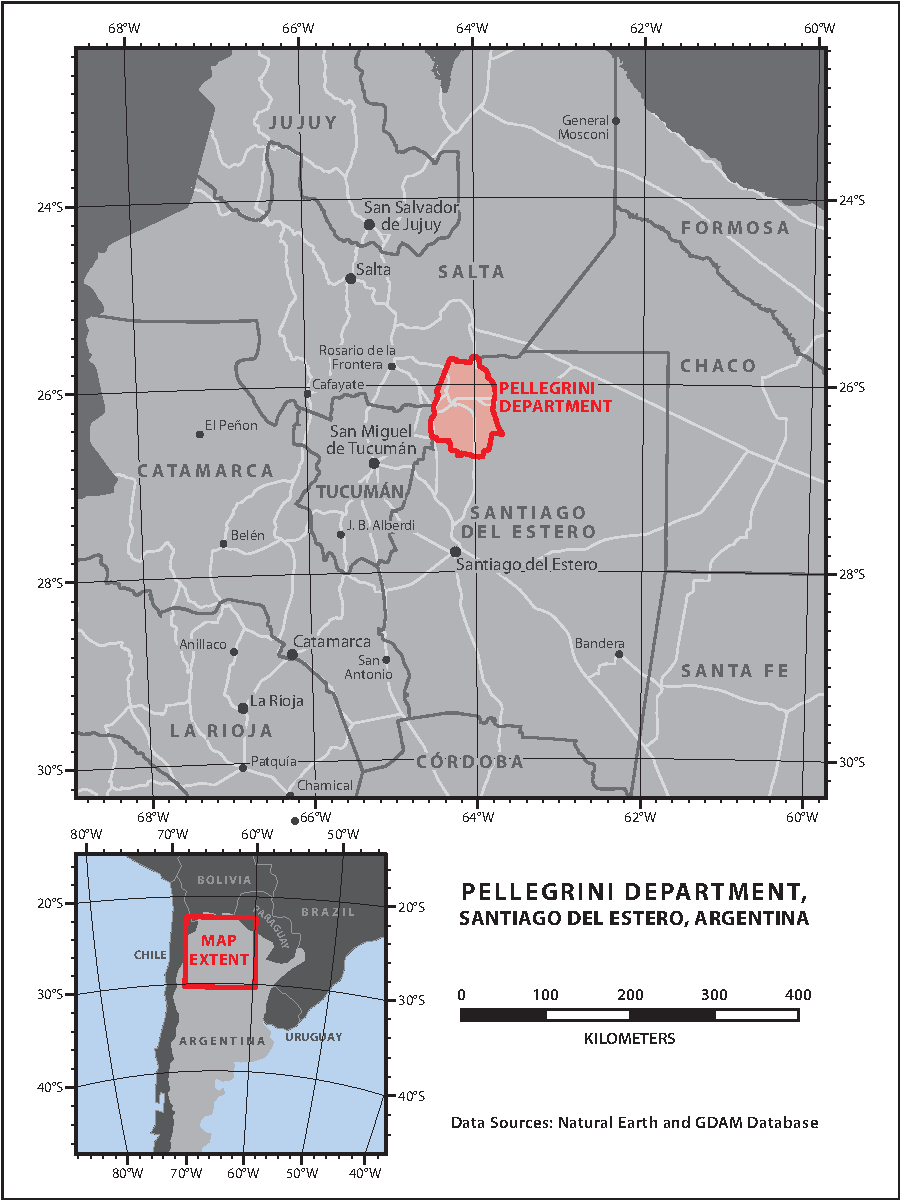
\includegraphics[width=\textwidth]{Graphics/argentinaOverview.pdf}
  \caption{The Department of Pellegrini and the Greater Northwest of Argentina}
  \label{map:argentinaOverview}
\end{ssfigure}

\begin{ssfigure}
  \centering
  \includegraphics[scale=.95]{Graphics/pellegrini75to14.pdf}
  \caption{Land Cover Change in Pellegrini from 1973 to 2014}
  \label{map:pellegriniCoverChange}
  \medskip
  \small
  These images show the progression of deforestation in Pellegrini. The lack of deforestation in the 1973-1975 composite is striking. As early as 1993, deforestation is visible, primarily in the Southwest along the RN34 highway. Little changed between 1993 and 2001, but by 2014 much more deforestation is visible throughout the entire area.\end{ssfigure}


\chapter{Data and Methods}
\label{chapter:methods}

\section{Overview}

The purpose of this study is to develop a set of tools to allow the classification of agricultural crops using a time series of imagery and known crop reference signatures and test the portability of the reference signatures. The data used for this study consists of the following:

\begin{Spacing}{1.2}
\begin{itemize}
  \item 250-meter MODIS 16-day Composite Vegetation Index images
  \item 30-meter 2012 USDA Cropland Data Layer (CDL): agricultural land cover raster dataset
  \item 30-meter Landsat 8 Operational Land Imager satellite imagery
  \item Shapefile of the administrative boundary of the Department of Pellegrini
  \item 2014 Land cover vector dataset with crop identifications for Pellegrini
\end{itemize}
\end{Spacing}

The first three datasets are publicly available from U.S. agencies. The Pellegrini boundary is from the GDAM Global Administrative Areas Dataset, version 1.0 (available at http://www.gdam.org). The land cover dataset for Pellegrini was digitized from Landsat 8 images (path 230, row 78), and the crop identifications were collected in the field.

An outline of the processing workflow is below:

\begin{Spacing}{1.2}
\begin{enumerate}
  \item Reproject the MODIS composite imagery
  \item Assemble individual composite images into single time series images, one for Kansas and one for Argentina
  \item Create a mask of all pure pixels (e.g. non-mixel) in the time series images
  \item Use the CDL to isolate the pure corn, soy, and sorghum pixels in the Kansas time series image.
  \item Identify the unique groups in each set of isolated pixels using k-means clustering
  \item Extract the pixel values for each cluster from the time series image and find the mean value for each date to find the unique signatures for each crop
  \item Validate the signatures by fitting the signatures to the time series image, then classifying the fit rasters to check the accuracy
  \item Fit the signatures to the Argentina time series image
  \item Classify the Argentina fit rasters and assess the accuracy
\end{enumerate}
\end{Spacing}

This chapter is a look at the theory and concepts behind this classification approach, the methods and fieldwork used to create the validation land cover dataset of Pellegrini, and the data processing steps used to generate the study results. Details about the specific tools in the classification toolset and the development process can be found in Appendix \ref{appendix:tools}. For a detailed explanation of all the testing proceeding this study, please see Appendix \ref{appendix:testing}. A thorough recounting of my field experience can be found in Appendix \ref{appendix:fieldwork}.


\section{Field Methods and Data Collection in Pellegrini}

While ground truth data was easily available for the Kansas study site, getting a ground truth dataset for verification of the classification in Pellegrini was not so simple. Such a dataset did not exist, necessitating onsite data collection. I visited Argentina mid-March to early April 2014 to gather field observations of summer crop types and to talk to local farmers about typical agricultural practices, summer and winter crop varieties, and planting and harvesting dates.

To guide my ground truth collection, I generated 400 random points inside the Pellegrini shapefile boundary, and used a Landsat OLI image as a reference for land cover (image date \formatdate{5}{2}{2014}). Where a point fell within a mixel, I allowed it to be moved within a 3-by-3 pixel window centered on the point's original pixel, trying as much as possible to keep the point within a pixel belonging to the feature type on which it originally fell. In certain limited cases, if a point fell quite obviously within a field but the center pixel and eight surrounding pixels were mixels and/or were not within the field, I allowed the point to be moved to the closest full pixel of that same continuous field. Of the 400 points, I had move 106 within the 3-by-3 window, and ten to a non-neighboring pixel within the same field.

The primary means of gathering the crop identities to complete the ground truth was direct observation. However, this strategy proved to be difficult in many cases; often, fields were not accessible due to road conditions or locked gated. Data not from direct observations came from interviews with farmers and land owners. In such cases, the interviewees were asked to identify their fields on printed maps with the reference Landsat imagery and describe their cultivars. The data from observations and interviews was recorded directly on the maps and later manually digitized.

Ancillary information about agricultural practices in the region was also collected whenever possible. It was a key goal to identify each crop's date range for planting and harvesting in order to allow the proper selection of MODIS imagery dates and setting of the $tshift$ bounds for Equation \ref{eq:gofx}.

\section{Data Processing}

\subsection{Resampling the CDL}

To use the CDL as a ground truth with the Kansas TSI, the 30-meter CDL pixels were resampled by majority to match the larger TSI pixels. This allowed a direct comparison between the crop values from the CDL and the pixel signatures in the TSI.

\subsection{Building the TSIs}

For this study, I chose to classify the 2012 Kansas summer growing season and the 2014 Argentina summer growing season. I assembled the MODIS 16-day composite VI images into multi-date time-series images (TSI) covering the growth cycle of the summer crops, where each band in a TSI is a 16-day composite VI and the bands are ordered consecutively (see Appendix \ref{appendix:tools:build} for the description of the Build Multidate Image Tools). The Kansas summer TSI covered the date range DOY 97 through DOY 273, and was made with data from the Terra satellite (LPDAAC product MOD13Q1, tile h10v05). Prior to creating the TSIs, each of the 16-day composites was reprojected from the native MODIS sinusoidal reference system using LPDAAC's MODIS Reprojection Tool \autocite{modis4.1}. I reprojected the Kansas data into the Albers Equal Area Conic projection for the contiguous USA using the 1983 North American Datum (WKID: 5070) to match the reference system of the USDA CDL.

In Argentina, as it is in the Southern Hemisphere and the seasons are inverted to those of the Northern hemisphere, the growing season shifts, as must the date range for the VI time-series. The TSI for Pellegrini must begin at the end of the proceeding year to adequately capture the entirety of the summer phenologies. To accomplish this, the time-series image for summer 2014 began with the 16-day composite image from DOY 353 of 2013 (or DOY −13 with reference to 2014) and ended with the image from DOY 161 of 2014 (MODIS grid tile h12v11). This specific date range was chosen based on information provided by local farmers to ensure coverage of the earliest planting and latest harvesting dates, as well as manual inspection of pixel signatures throughout the study area. Persistent clouds necessitated using an image from the Aqua satellite of DOY 105 (LPDAAC product MYD13Q1) in place of DOY 113 from Terra. Due to no viable imagery from Aqua or Terra, DOY 129 was interpolated via a simple mean from the DOY 105 Aqua image and the DOY 145 Terra image. The Argentina composite images were reprojected with the UTM Zone 20S reference system (WKID: 32720).

\subsection{Eliminating Mixels}

After building the TSIs, the next processing step was to eliminate mixels from the TSIs, to prevent errors caused by mixed temporal signatures (see Appendix \ref{appendix:testing:r2} for more information). Pure pixels, the non-mixels in an image, were isolated by intersecting the ground truth datasets with a vector grid of the TSI pixels. Then, all pixels with an area greater than an area threshold were selected as pure. Only these pure pixels were classified; the mixels in the TSIs were excluded.

The original 30-meter CDL raster served as the reference for finding the pure pixels in the Kansas study site. The raster was converted to vector polygons and intersected with the TSI grid polygons. From the resulting geometry, all polygons greater than 53,000 square meters (or 98 percent of a full MODIS pixel) were selected as pure. I also manually selected two sorghum pixel features that were omitted due to intermixed soy pixels. I chose to add these pixels due to the low number of sorghum features retained, and that the intermixed soy appeared to be errors.

For the Argentina analysis, the digitized features of identified fields were combined with manually digitized features of all large forested areas, unknown fields, and ``other'' areas. Some places where the land cover was mixed and could not be visually differentiated were not digitized and were considered to be composed entirely of mixels. The complete dataset of land cover was then intersected with the Argentina TSI grid. Through trial and error, a minimum area of 50,000 square meters was chosen as the threshold for pure pixels in the image.

\subsection{Extracting the Reference Temporal Signatures}

As a reference library of temporal signatures does not yet exist, I had to extract my own signatures from the Kansas TSI. To do so, the pure TSI pixels of each key summer crop---corn, soy, and sorghum---as specified in the resampled CDL were isolated in separate rasters. Each of separated rasters was clustered into three clusters using the ENVI \autocite{envi5.0} k-means tool with a 1.0 percent change threshold over 100 maximum iterations. The TSI pixels in each cluster were then sampled and averaged to find the three primary signatures for each crop\footnote{Given the existing literature about phenological classification, I do not believe crops have multiple signatures. I believe every crop as a theoretical ideal signature, which can be made to fit any actual signature using the $xscale$, $yscale$, and $tshift$ transformations in Equation \ref{eq:gofx}, barring any unusual effects of weather or other forces impacting crop development (a mid-season drought, for example, may cause a crop signature with double peaks due to the partial dying off and regeneration of the plants). However, given my choice of the CDL as my source of ground truth, I have had to make the assumption that it is highly accurate, despite any evidence to the contrary (see my discussion of the CDL beginning in \autoref{appendix:testing:r3}). Therefore, I use the clustering to derive the signatures that will create a classification most comparable to the CDL.} (see \autoref{appendix:tools:extract} for information about the Extract Signatures Tool).

\subsection{Fitting the Reference Signatures to the TSIs}

\autoref{eq:1} (page \pageref{eq:1}) was implemented using the programming language Python \autocite{python2.7.8} with a command line interface to allow easy processing of the TSIs. Details of the tool can be found in \autoref{appendix:tools:fit} on page \pageref{appendix:tools:fit}. The tool iterates through every pixel in a TSI, comparing each reference signature with the pixel signature. The tool is able clip an input TSI to either pixel bounds or a shapefile containing a polygon, and can also use an optional point shapefile to limit the processed pixels to only those coincident with points. An output raster is created for each signature to record the RMSE from every pixel comparison.

The reference signatures extracted from the Kansas TSI clusters were fit to the Kansas TSI to verify the classifier. The TSI was clipped to pixel row 2482 and column 1089, extending 100 rows and 100 columns. Then, the same Kansas signatures were fit to the Pellegrini TSI, which was clipped to the boundary shapefile. The fit rasters from each TSI were then classified. In both cases, the bounds for the $xscale$ and $yscale$ parameters were 0.6 to 1.4. The $tshift$ bounds for the Kansas processing were -10 to +10 days, while the bounds for the Pellegrini processing were 120 to 140 days (still $\pm10$ days, but shifted 130 days).\footnote{I have not formally tested other bounds. See Appendix \ref{appendix:future:fitting}.}

\subsection{Classifying the Fit Rasters}

The classification process is complex; Appendix \ref{appendix:tools:classify} contains a full discussion of the process, so I will refrain from a lengthy description here.

Classifying the fit rasters first requires thresholding the values in each raster, then finding the lowest value for each pixel. The signature with the lowest thresholded fit value has the best fit, and the pixel is classified as that crop. The thresholding prevents pixels with poor fit values from being classified as a crop. If a pixel has no remaining fit values after thresholding, it is classified as ``other.'' Currently, appropriate threshold values are not well understood, so to find the best classification, the classification tool must brute-force through many combinations of thresholds within a user-specified range, classifying the fit rasters, and calculating the accuracy of each threshold combination in comparison with the ground truth dataset. A raster of the classification with the best accuracy is retained.

For the Kansas classification, it was easy to try iterating through different threshold ranges. However, the Argentina classification was not as straightforward. As the tool must brute-force through every threshold combination, the time required to find the best threshold in a range is exponential, given by the number of threshold steps to the power of the number of images, times the number of seconds for each iteration. The Kansas classification took under 0.3 seconds per iteration; classifying the larger area of Pellegrini took substantially more time, somewhere between three and four seconds per iteration. The increased processing time ruled out using more than two or three steps in any given iteration. Consequently, in the case of the Argentina classification, I found it much more efficient to iterate through a range of threshold values using a single threshold value across all the fit rasters, then manually refine the thresholds until a suitable threshold combination was found.
%\chapter{Timeline}

I hope to have finished the classification algorithm by the beginning of winter term 2014.  At that point, I will run the testing on the Kansas sample areas to find the best reference curves. Once that testing is completed, I will use those curves to classify MODIS data of Pellegrini from the 2012 -- 2013 growing season. This will provide me with a rough picture of the crop cover my method will find for 2013 -- 2014, and from this I can use a stratified random sampling technique to better ensure my ground truthing will contain sufficient sample points in each land cover class. In March 2014 I plan to do fieldwork in Pellegrini to collect the ground truth data for these points. I have chosen the month of March specifically because it is in the middle of the summer growing season, and I can get ground truth data for summer crop identification as the crops are growing. Winter crops, such as winter wheat, will need to be verified by inquiring with field owners, or confirmed by visual interpretation of Landsat imagery. In spring term 2014, I will classify 2013 -- 2014 data for Pellegrini, calculate the accuracy using the ground truth acquired in March, and begin writing. I plan to finish my work and writing over summer 2014 and present fall 2014.

\chapter{Results}
\section*{Preliminary Results}
\label{sec:prelim}

To this point, I have been able to create scripts to import and assemble my multi-date images; to sample images and generate mean reference curves of the VI values for soy, corn, and wheat (Fig. \ref{fig:curves}; and to take said reference curves and generate an image for each crop, of which the pixel values are the RMSE after constrained minimization, and an image with the best fit for each pixel (Fig. \ref{fig:testing1}). For script development I am using MODIS 16-day EVI data from 2012. I have not completed the computation of the confidence scores of any given classification (a la fuzzy classification), but, for the sake of exploring this initial output, I used a threshold of .08 RMSE and classified the image according to the best fit. That is, for any pixels which had an RMSE of .08 or less for one or more of the crops tested, I used the best fit image values for those pixels as the values for classification (Fig. \ref{subfig:classification1}). I used the USDA CDL for 2012, resampled to 250 meter pixels with the majority value (Fig. \ref{subfig:CDL}), to check my classification. Building a confusion matrix for all of the pixels in the image resulted in Table \ref{table:acc}. As shown, the accuracies for each of the crops ranged between 60 percent and 70 percent, with an overall accuracy of 63 percent, though the kappa value is somewhat low at 0.44. Nonetheless, considering this is the unoptimized algorithm with an arbitrary threshold value, I believe my results suggest this classification method to have potential.

\begin{figure}
  \centering
  \includegraphics[width=\textwidth]{Graphics/cropCurves.pdf}
  \caption{Mean phenological curves found for corn, soy, and winter wheat. Each curve is generated from the mean EVI values of four pixels of the respective crop from an initial test area in 2012 Kansas data.}
  \label{fig:curves}
\end{figure}

\begin{figure}
  \centering
  \begin{subfigure}[b]{.45\textwidth}
    \includegraphics[width=\textwidth]{Graphics/corn1_edited.png}
    \caption{Fit of corn reference curve.}
    \label{subfig:corn1}
  \end{subfigure}
  \quad
  \begin{subfigure}[b]{.45\textwidth}
    \includegraphics[width=\textwidth]{Graphics/soy1_edited.png}
    \caption{Fit of soy reference curve.}
    \label{subfig:soy1}
  \end{subfigure}
  \\
  \vspace{.25in}
  \begin{subfigure}[b]{.45\textwidth}
    \includegraphics[width=\textwidth]{Graphics/wheat1_edited.png}
    \caption{Fit of wheat reference curve.}
    \label{subfig:wheat1}
  \end{subfigure}
  \quad
  \begin{subfigure}[b]{.45\textwidth}
    \includegraphics[width=\textwidth]{Graphics/bestfit_edited.png}
    \caption{Best fit image.}
    \label{subfig:bestfit1}
  \end{subfigure}
  \caption{Initial test results.}
  \label{fig:testing1}
\end{figure}


\begin{figure}
  \centering
  \begin{subfigure}[b]{.45\textwidth}
    \includegraphics[width=\textwidth]{Graphics/classification1_edited.png}
    \caption{Initial classification of corn, soy, and wheat.}
    \begin{minipage}{.1cm} %fills vertical space to vertical align both subfigures
      \vfill
    \end{minipage}
    \label{subfig:classification1}
  \end{subfigure}
  \quad
  \begin{subfigure}[b]{.45\textwidth}
    \includegraphics[width=\textwidth]{Graphics/cdl_rsmp_edited.png}
    \caption{2012 USDA CDL, resampled to 250m pixels to match MODIS data.}
    \label{subfig:CDL}
  \end{subfigure}
  \caption{Initial classification and ground truth}
  \label{fig:classification}
\end{figure}


\begin{table}
  \centering
  \caption{Accuracy assessment of the initial results.}
  \label{table:acc}
  \begin{tabular}{rcccccc}
    \toprule
     & Corn & Soy & Wheat & Other & Total & User Accuracy \\
    \midrule
    Corn & 260 & 22 & 6 & 103 & 391 & 67\% \\
    Soy & 10 & 59 & 1 & 29 & 99 & 60\% \\
    Wheat & 33 & 0 & 354 & 127 & 514 & 69\% \\
    Other & 174 & 27 & 241 & 670 & 1112 & 60\% \\
    Total & 477 & 108 & 602 & 929 & 2116 \\
    Producer Accuracy & 55\% & 55\% & 59\% & 72\% \\
     &  &  &  &  &  & Overall: 63\%\\
     &  &  &  &  &  & Kappa: 0.443 \\      
    \bottomrule
  \end{tabular}
\end{table}


\section*{Anticipated Outcomes}

Upon the completion of my research, I expect to have a working tool which can be used as an economical and effective means of crop classification. With the results of my testing, I will know how changes in the generation of the reference curves effects the results of the classifier. Using this tool and knowledge, I will generate crop maps of my study areas, and quantify their accuracies. The results of this study should be of value to those working in the field of remote sensing and those investigating LULC change, particularly in regard to deforestation and agriculture. I hope this work will be the basis for future investigations into soy's role in Argentina's deforestation.



















\chapter{Discussion}
\label{discussion}

\section{Examining the Kansas Signatures}
\label{discussion:kssigs}

The Kansas signatures extracted from the k-means clusters (\autoref{fig:KScropsigs}) were not as variable as I was expecting. Based on some initial testing results, presented in \autoref{appendix:testing:r3} beginning on \autopageref{appendix:testing:r3}, I expected to find some strange looking cluster signatures. Aside from the Soy\_1 signature, and perhaps the Corn\_1 signature to some degree, the cluster signatures were fairly typical in appearance. The Sorghum\_1 signature appears more or less as expected over the TSI's date range, but does seem to be missing the late-season downslope.

Using the k-means algorithm to cluster each crop's pixels might not have adequately captured the variability in the crop signatures as labeled by the CDL to allow the fit algorithm to match the CDL classification. That is, perhaps k-means separates pixels that would have similar RMSE values when fit with the same crop reference signature. Future research might want to consider clustering based on the RMSE value of each pixel to the others; pixels with low RMSE values when compared to one another would be grouped together, as they likely to be transformations of the same base temporal signature. Pixels with considerably different RMSE values would suggest different base temporal signatures.

Despite the fact the k-means might not capture similarity in the same way as the fit algorithm, it is worth noting that the k-means clusters do not divide any fields: each pixel in a field is assigned the same cluster (\autoref{map:KSclusters}). This result shows that each pixel in a field of multiple pixels typically has a similar signature to all the others in the field, at least using k-means as a measure of similarity. This result is further confirmation of the hypothesis that each pixel of a crop that grew under the same conditions, such as a field, should have the same development and therefore same temporal signature.

\section{Breakdown of the Kansas Classification}
\label{discussion:ksclassification}

The initial verification of the Kansas reference signatures, done by classifying the TSI of the Kansas study area, demonstrated the method performs well when used to match the original source data (\autoref{table:ksresults}). The 84.4 percent overall accuracy and kappa value of 0.76 are well within the range considered acceptable, especially given the CDL's published accuracy of 88.4 percent (to which this classification is compared).

Some confusion between corn and soy, as well as soy and ``other,'' pulled down the overall accuracy, as well as the producer and user accuracies of each of those classes. The similarities between the corn and soy signatures may cause late corn and early soy to be confused if the range of the offset of the beginning day of the reference signature, $tshift$, allows overlap between the two. I believe much of the soy and ``other'' confusion was due to the Soy\_1 reference signature (\autoref{fig:KScropsigs}). Examining the CDL classes of the best fit pixels in the RMSE raster showed a number of grassland pixels were well fit by that particular signature. However, omitting that particular signature seemed to allow one of the corn signatures to take many of the soy pixels, which I find strange due to the peculiar shape of the Soy\_1 signature. In fact, the signature does not match the traditional soy signature, and makes me question the validity of the CDL in this case (also see \autoref{appendix:testing:r3} for more CDL problems, and \autoref{appendix:cdl} for notes about the CDL).

Classifying sorghum did not seem to be very effective; only two of the 18 sorghum pixels were accurately identified. The sorghum RMSE raster had the lowest threshold value at 450, but increasing the threshold only caused greater class confusion. Omitting the signature entirely had a slight negative effect on the overall accuracy, as the ``other'' pixels it misclassifies would otherwise be misclassified by corn and soy. It is possible that I should have added another 16-day composite to the TSI to capture the tail-end of the sorghum signature, though I believe doing so would have caused more harm as winter crop plantings would begin to interfere with summer crop signatures (see the ``end-of-year bump'' discussion in \autoref{appendix:testing:r4}). Moreover, the similarities between sorghum and soy signatures might cause confusion if the sorghum threshold were to be raised. However, due to the low number of sorghum pixels, the validity of any conclusions about classifying this particular crop is questionable. A larger sample size and more testing are required.

\section{The Pellegrini Classification and Class Confusion}

As shown in \autoref{map:ARclassification}, classifying the Argentina TSI with the reference signatures from the k-means clustering of the Kansas TSI was able to effectively separate areas of the summer crops corn, soy, sorghum, and poroto from most other land cover classes, but classified those summer crop pixels predominately as as corn. While \autoref{table:ARbestresult} reflects this class confusion in the producer and user accuracies, the low sample count for corn, soy, and sorghum compared to all the other land covers deceptively skews the overall accuracy higher. \autoref{table:ARpurepxresults} is the confusion matrix for the same classification, but compared to the entire ground truth dataset, encompassing some 85,821 pixels, instead of the rather limited 378 random sample points. While the overall accuracy actually improves slightly with this new reference dataset, it must be noted that neither of these accuracy assessments is able to account for errors resulting from mixels. However, the increased number of samples better demonstrates the significant corn-soy confusion. For instance, of the 6,621 pixels classified as corn, 2,076 are soy. Errors of omission are also more prominent: 2,234 of the 5,706 corn pixels were left as ``other.'' A similar proportion of soy pixels were also classified ``other.'' Increasing the RMSE thresholds on the RMSE rasters to decrease these omissions only increased the errors of commission, confusing ``other'' pixels for crops. The low kappa statistic of both accuracy assessments, 0.54 and 0.51 respectively, is reflective of the poor accuracies within the summer crops.

\begin{sstable}
  \centering
  \caption{Summer 2014 Pellegrini Best Classification Accuracy Checked Against All Pure Pixels}
  \label{table:ARpurepxresults}
  \begin{tabu}{rrrrrrrl}
    \toprule
     & & \multicolumn{4}{c}{\textbf{Reference Data}} & & \\
     &  & Corn & Soy & Sorghum & Other & Total & User Acc. \\
    \midrule
    \multirow{4}{*}{\rotatebox{90}{\textbf{Classified}}} & Corn & 3283 & 2076 & 61 & 1201 & 6621 & 49.58\% \\
     & Soy & 189 & 313 & 36 & 458 & 996 & 31.43\% \\
     & Sorghum & 0 & 0 & 0 & 0 & 0 & 0.00\% \\
     & Other & 2234 & 1523 & 60 & 74387 & 78204 & 95.12\% \\
     & Total & 5706 & 3912 & 157 & 76046 & 85821 &  \\
     & Producer Acc. & 57.54\% & 8.00\% & 0.00\% & 97.82\% &  &  \\
    \multicolumn{8}{r}{Overall Accuracy: 90.87\%} \\
    \multicolumn{8}{r}{Kappa: 0.51} \\
    \bottomrule
  \end{tabu}
\end{sstable}

Considering that the ``other'' pixels contain a number of different classes, I found the frequency of corn and soy classifications within each of the ``other'' land cover classes. The results of this analysis (\autoref{table:ARotherconfusion}) show that the main sources of confusion were, from greatest to least, the true ``other land cover'' class, pasture, and poroto. However, when finding the percent of the land cover class pixels that were confused, poroto leads with over 26 percent of its pixels confused for either corn or soy. This confusion, and the confusion of some pasture areas as well, does make some sense, as these land covers, soy, and corn are all planted in spring and reach peak maturation during the summer months. Depending on the type of pasture, it may or may not grow back after cutting; if it does not, the temporal signature may bear some resemblance to corn or soy.\footnote{I heard a few names for a few different types of pasture grasses that were being grown in the area, but I believe the two most prevalent are known locally as \textit{\textspanish{gatom pani}} and \textit{\textspanish{grama}}. I have not been able to determine if \textit{\textspanish{gatom pani}} has an english name; it is possible that I did not get the correct spelling. Blue Grama Grass (textit{Bouteloua gracilis}) is a common forage grass native to North America, though I am unsure if it is the same plant grown in Pellegrini. I did not learn much about any other pasture grasses cultivated in the area, or about typical harvesting practices.}

\begin{table}[b]
  \begin{Spacing}{1.0}
  \centering
  \caption{Pellegrini Corn and Soy Confusion with ``Other'' Land Cover Classes}
  \label{table:ARotherconfusion}
  \begin{tabu}{X[0.6,m,c]X[0.5,m,c]|X[1,m,c]X[0.55,m,c]|X[1,m,c]X[0.55,m,c]}
    \toprule
    \textbf{Land Cover} & \textbf{Total Pixels} & \textbf{Confused as Corn} & \textbf{Percent of Total} & \textbf{Confused as Soy} & \textbf{Percent of Total} \\
    \midrule
    Forested & 63,978 & 194 & 0.30 & 26 & 0.04 \\
    Other & 5,393 & 306 & 5.67 & 322 & 5.97 \\
    Pasture & 5,252 & 396 & 7.54 & 50 & 0.95 \\
    Poroto & 1,369 & 303 & 22.13 & 59 & 4.31 \\
    Nothing & 485 & 2 & 0.41 & 1 & 0.21 \\
    \bottomrule
  \end{tabu}
  \end{Spacing}
\end{table}

From their appearance in Landsat imagery, the main locations where the other class was confused for corn and soy seem to be bare earth, possibly due to high soil salinity. The areas have low-to-moderate reflectivity in the visual bands, high reflectivity in the mid-infrared, and low reflectivity in the near-infrared, and do not exhibit much change over time. However, the plots of a random sampling of pixels from the TSI show temporal signatures like that in \autoref{fig:ARweirdsig}.
I am currently unable to explain what is in these areas or why they are confused for corn and soy. I believe there may be some sort of summer grass cover or other seasonal vegetation, but I cannot understand the lack of near-infrared reflectance as observed in Landsat images from multiple dates throughout the summer.

\begin{ssfigure}
  \centering
  \input{plots/strangepoint1.pgf}
  \caption{Signature of an Unknown Pixel Confused for Corn and Soy in Pellegrini}
  \label{fig:ARweirdsig}
\end{ssfigure}


\section{Clustering Pellegrini}

To further examine the class confusion in Pellegrini, I used the same k-means clustering as in Kansas to identify the three main signatures for each of the eight land cover classes in the ground truth dataset. The extracted corn, soy, and sorghum signatures are shown in \autoref{fig:ARcropsigs}, while the poroto and pasture signatures are in \autoref{fig:ARporotopasturesigs}.

The cause of the corn-soy confusion is immediately visible: both crops peak around the same date. I did not expect this result, as the typical planting dates I collected suggest soy should peak earlier than corn.\footnote{Even if soy had peaked earlier than corn, I would not have been able to achieve an accurate classification with the current tools, as corn-before-soy is a key assumption. That is, a single $tshift$ parameter is specified for all reference signatures. It would be possible to rewrite the tool to allow different $tshift$ values for different signatures, which might have sufficed if soy did peak before corn, but does not help when the peaks are coincident.} However, I also gathered that precipitation was the limiting factor in planting (confirmed by \autocite{sacks2010crop}), and often farmers will wait until a certain amount of rain has fallen before planting. In fact, I was told the rains this year were quite late, and on multiple occasions farmers told me they had planted a field late due to lack of rain. While I must admit I am not a farmer and do not know this for certain, the reason for waiting did not seem to be out of concern for plant health, in that too early of planting would negatively impact the crop's health, but seemed to be primarily economic: farmers do not want to pay to plant crops that will not grow if the rains never come.

\begin{ssfigure}
  \centering
  \input{plots/cropsigsAR.pgf}
  \caption{Corn, Soy, and Sorghum Signatures Extracted from the Pellegrini TSI}
  \medskip
  \small
  These are the signatures from the k-means crop clusters found in the Pellegrini TSI. While some strange exceptions like Soy\_3, Sorghum\_1, and Sorghum\_3 deviate from the rest, the overwhelming similarities between signatures of different crops is striking. Unlike the crop signatures from Kansas, Pellegrini's crops are not temporally separated, but peak almost simultaneously.
  \label{fig:ARcropsigs}
\end{ssfigure}

\begin{ssfigure}
  \centering
  \input{plots/poroto_pasture_sigsAR.pgf}
  \caption{Poroto and Pasture Signatures Extracted from the Pellegrini TSI}
  \label{fig:ARporotopasturesigs}
\end{ssfigure}
The forest, nothing, and other signatures are in \autoref{fig:ARothersigs}.

\begin{ssfigure}
  \centering
  \input{plots/othersigsAR.pgf}
  \caption{Forested, ``Nothing,'' and ``Other'' Signatures Extracted from the Pellegrini TSI}
  \label{fig:ARothersigs}
\end{ssfigure}

I also observed fields of corn, soy, sorghum, and poroto in many different states of development, from the early, barely-germinated stage to the late, fruit-bearing stage. To me, the broad range of development is likely because water is the only limiting factor defining the typical planting dates. That is, the threat of changing temperatures does not affect planting decisions like in Kansas, and farmers have much more flexibility (this flexibility has been observed in other regions per \textcite{sacks2010crop}). Additionally, early and late planted crops should mature about the same time, due to their development being limited by water. My method should be able to accommodate the range of planting and maturation dates by adjusting the bounds on the $tshift$ parameter, allowing the reference signatures more freedom to temporally align themselves with the pixel values. However, there is one problem with that idea: my method deals with similar-looking signatures, like corn and soy, by making an assumption that each should peak within different time ranges. In Kansas, corn peaks before soy, and as such they can be differentiated. Planting dates for Argentina as a whole also suggest corn should peak before soy. However, in Pellegrini specifically, the weather conditions and consequent agricultural practices do not allow this assumption to be met. When both crops peak about the same date, their temporal signatures are not significantly different, leading to the class confusion exhibited.

I believe higher temporal resolution data might create more detailed temporal signatures, which could allow for more difference to be detected between different crops. Combining such data with certain noise-filtering methods may allow signatures to be smoothed in ways that might accentuate differences between similar crops like corn and soy (see \textcite{doraiswamy2006improved} and \textcite{sakamoto2010a-two-step} for examples of higher temporal resolution data and filtering).

\appendix
\chapter{The Story of My Field Work}
\label{appendix:fieldwork}

In order to complete an accuracy assessment of the classification I was to produce of agriculture in Pellegrini, I knew I needed ground truth data with which I could compare my results. As I suspected would be the case, I was unable to find any extant datasets, so I knew I would have to visit Pellegrini to gather such data.

After extensively reviewing satellite imagery of the area, I knew the fields were very large and appeared to have many roads connecting them, so I did not expect access to be problematic. While the size of the department, 6,943 square kilometers, is about the size of Delaware, I thought I would be able to cover ground fairly quickly, and allocated three weeks of time in Pellegrini to gather all my data.

I did have concerns to how the local people would take to my project. I know that I would be immediately suspicious of some foreigner coming in to my town and wanting to know everything about the agricultural practices in the area, including visiting all of the fields. I actually practiced how to say, in Spanish, ``Don’t shoot! I am leaving, there is no problem.'' Perhaps this is just an American thing, but I was expecting, at some point, to be confronted by someone with a gun who did not like me. After all, I am not necessarily in favor of the agriculture that is taking over the area, and while I tried to present my views as neutrally as possible, I thought a conflict would be inevitable.

I arranged for a small rental car in San Miguel de Tucumán, Tucumán, a city about 150 kilometers from Nueva Esparanza. I knew the roads would not be great, but I figured I should be able to get through just about anything with the rental car, except mud. Nueva Esparanza was to be my base, and my plan was to try and visit the furthest areas first, as I expected those to the most difficult to access, leaving the easier areas for last.

As mentioned in my methods, I randomly generated 400 points throughout the department to survey. Of those 400, I immediately identified 247 of them as forested using Landsat imagery, which meant I did not need to visit them. For the remaining 153 I did need to visit, I created map sheets—one for every point, centered on the point—showing the point at three different scales: an overview at 1:60,000 scale, a closer image at 1:30,000 scale with the MODIS pixel grid overlaid, and a very large scale 1:4,500 scale view with older but higher resolution imagery from Digital Globe. I also created a 25-kilometer grid over Pellegrini, which I used to make eighteen smaller-scale ``regional'' maps at 1:150,000 scale to help identify neighboring points and plan routes. Lastly, I made an overview map of the entire department at 1:475,000 scale. I printed all of these maps and put them in a binder. I planned to collect data about as many fields as I could, even those without sample points, and I got metallic markers so I could outline each field on the maps and take notes of crop types.

Getting to Nueva Esparanza was a challenge in itself. Due to the budget fare the airline provided me in exchange for my miles, it took me some 36 hours just to get to the hostel in Buenos Aires. Once there, I had to make my way around town to gather some supplies and change money. I had a short night in the hostel, as I needed to make an early flight from Buenos Aires to San Miguel de Tucumán. I picked up my rental car at the airport in Tucumán, at which point my stress level increased significantly, as I now had to make my way around the city not as a passenger, but as a driver. Argentine traffic laws do exist, but my perception is that, generally speaking, no one knows what they are.

Another problem was gas. Even something as simple as purchasing fuel for one’s vehicle can become a new and stressful experience in a foreign country. After visiting Guatemala, where drivers would pull up to random buildings around town and attendants would appear from nowhere with a container of gasoline and a makeshift funnel made from the top of a plastic bottle, I was unsure what to expect. It turned out that the process was not so rudimentary nor much different from buying fuel back home, and my concern was mostly unwarranted.

After driving throughout the city gathering supplies, it was time for me to head to Nueva Esparanza. Despite using two maps and my GPS to try and navigate my way to the correct highway, I found myself on the wrong road out of town, and had to spend an inordinate amount of time following a long string of slow moving cars along what seemed more to be a series of main streets through a corridor of small towns than a highway. Thankfully, however, the road eventually led to the route I initially intended to take, and I began to make more rapid progress towards Nueva Esparanza.
Unfortunately, my rapid progress quickly slowed upon reaching the beginning of road construction, which persisted the next 70 km or so.

My first full day I was in Nueva Esparanza I planned out a long route to investigate, but, after talking with some of the workers of the hotel I was staying in about my security concerns, I decided I should visit the police \textit{comisaria} to ask if I was going to have any problems with land owners or locals while working. The first moment I opened my mouth I became the attention of everyone in building. I used the best Spanish I could muster to try to tell them what I was there to do and why, but I kept getting passed from person to person. Eventually, based on the questions they were asking me—things I was sure I had already said—I realized they could not understand me. And I was struggling mightily myself to understand them.

After some two and a half hours and what must have been forty people trying to interviewing me, the police were finally able to track down an English teacher who taught in the local schools. With his assistance, I was able to communicate the details of my project, and the police made up an official document vouching for my identity and purpose in case anyone took issue with my presence in the department. Everyone assured me that I would not have any problems with the people. Not once during my trip did I need the document.

In spite of the late hour I left the police station that first day, I naïvely attempted to complete the long route I had laid out for myself. My early progress was actually quite good; I did not check off many points, but I was able to visit quite a number of fields in a short amount of time. This served only to errantly bolster my self-confidence.

In line with my plan to visit the furthest points first, I was making my way to the far northwest corner of Pellegrini. About an hour and a half from Nueva Esparanza, I came to the border with the province of Salta. Looking at the Landsat imagery, I could clearly make out a long, straight road following this line. That this road was not marked on any other maps should have been a clue to me.

After a few minutes of searching and considering the numerous side paths along the main road, I determined the correct road to follow, and proceeded to head north along it. I had a thought about the sandiness of the road, but knew that as long as I maintained my momentum I should not have any problems. I did not consider the hour, which was closing in on 5:00 PM, nor the fact that, due to my lengthly visit with the police, I had not taken the time to eat that day, aside from a breakfast consisting only of a banana.

Only a few minutes down the road, the situation quickly worsened. Deep ruts suddenly appeared in the middle of the road, and I did my best to straddle the car over the left one by attempting to drive with my left tires on the side of the road and my right tires down the middle. However, the success of this maneuver was short lived, and before I knew it, the small, low car had dropped down into the ruts. I stepped on the gas, hoping that keeping the car moving would keep me for getting stuck. The sound of the sand scraping at the underside of the car was unbearable. I spotted a break in the vegetation on the left side of the road, so I pointed the car at it, hoping the wheels would be able to break free from the ruts with a sharp enough turn. Luckily, this time my maneuvering was successful, and I found myself parked on the only hard patch of clear ground in visible surroundings.

I got out of the car and surveyed the situation. The deep, sandy ruts continued in both directions along the road. Being only a few minutes from the main road, and realizing the lateness of the hour, I figured the only reasonable course of action would be to return to Nueva Esparanza. I contemplated driving through the small brush along the side of the road to get back to where the ruts were shallower, but I figured my tires would have been no match to the large thorns common to so many of the Chaco’s plants. My only regress would be to attempt to drive back the way I came.

Careful of the thorniest of plants, I managed to turn my car around, orienting it in the proper direction. I knew I needed to do two things if I were to make it back to the main road without problems: go fast, and stay out of the ruts. I was able to do neither.

I stepped on the gas, but given the gearing of the Chevy and its abysmally-small power plant, quick of the line it was not. Adding to the fact that I was wholly unsuccessful at keeping out of the ruts, I managed all of three or four meters before losing all forward momentum. I tried rocking the car by repeatedly shifting between first and reverse, but only managed to get the car more firmly planted in the sand.

Thanks to the sound advice of Polo, one of my committee members, I had actually purchased a shovel the day before in Tucumán. To say that at this point the shove came in handy would be an understatement.

I proceeded to dig out all the sand underneath the car upon which it was high centered, as well as a short path both in front and behind the car, and attempted another run at freedom. I repeated these steps numerous times with no success. Each time I felt that much closer to collapse due my plummeting blood sugar.

Some time into this cycle a woman approached on a motorcycle with her two kids. I stood there, staring at her as she drew closer, hoping she would stop and tell me she would be right back with someone to help me out. Instead, she stopped and began looking at me as if amused as I proceeded to explain my predicament as best I could. She told me in the most unhopeful manner that she would send someone my way, if she found anyone who could help. I still wonder what became of that woman and her two kids.

Eventually, I became wise to my insanity, and decided I needed to try another course of action. I recognized my problem was acceleration: each time I tried to accelerate, my tires would dig into the sand, and the ruts would present themselves as that much deeper. In order to escape the situation, I needed to be able to get my car to speed before I encountered any ruts.

I quickly went to work regrading a 30 meter length of road. By this point I was on the verge of passing out, but I knew I could not take a break. Even if it had dawned on me that I could have eaten one of my cup of noodles raw (the only food I had in the car due to a misjudgment in preparation for this day trip) I could not have stopped to do so, as I needed to get myself out before dark or I would be stuck there all night.

After what I estimate to be two hours of hard work in that energy-sucking heat, I finally managed to clear what I hoped would be a long enough section of road to get me free. Getting back into my car, I resigned myself to spending the night out there, my cynicism taking hold and condemning me an attitude of hopelessness. Yet, in spite of my natural inclination for pessimism, I found my car floating over the sand, making its way toward freedom. I did not let of the accelerator until I was sure I was free of the clutches of the sand, which, looking back, actually may not have been until I was safely parked outside my hotel.

At this point I knew my whole plan was falling apart. I had planned to visit some twenty-five points that afternoon, yet I only made it to four. I thought I could depend on myself to get around, but I realized my car was woefully incapable of passing all but the most traveled of roads. Moreover, many of the “roads” I had spotted on the satellite imagery and was depending on to get to my points were not in fact roads, but private paths behind fences, gates, and rows of bushes, accessible only to those with the permission of the landowner.

Even the roads that were accessible were beyond my worst nightmare. Perhaps my definition of bad was inaccurate; even when people told me before my trip the roads would be bad, I just said I’d be fine. I’ve driven on bad roads; what could be the problem? This is not to say I did not expect to have \textit{any} problems with the roads, but to see the condition of the main roads—all potholed, rutted, sandy, and muddy—and to get stuck on my first day out, was a humbling and troubling experience.

I needed help.

The road conditions were not the only reason either. My interactions with the police officers at the comisaría should have been a clue to the difficulty I would have communicating. Argentine Spanish is particularly difficult on its own (if one has learned Mexican and Central American Spanish as I have), but the Spanish in Pellegrini is another dialect entirely. Take Argentine Spanish and add indigenous terms and the accent and idioms of an isolated rural area, and I felt like I was trying to learn another whole language. If I could have chosen one thing to have made my trip smoother, it would have been a better command of Pellegrini Spanish. I was able to get by, and came to understand some individuals fairly well, but often I found myself unable to communicate effectively.

I became clear to me that I needed to break out of my comfort zone and rely on others. Doing so was very hard for me, as I tend to be extremely independent and like to do everything myself. I set unreasonably high standards, and few, including myself, can live up to them. However, I was clearly not succeeding on my own; I needed people that could get me to the places I had to see. It turned out that the English teach just so happened to have a motorcycle, and graciously agreed to take me out to survey points in the afternoons when he had free time. He also introduced me to a local teenager, who, despite his age, proved to be a worthy guide, as he knew the area and some English. His grandfather also had a truck, which helped us get around.

In working with these guides, I quickly came to learn that I was going to have the best success not in going to every survey point myself, but in talking with local farm hands and landowners. Even with the right vehicle, many places were still inaccessible, primarily because many “roads” on the satellite imagery didn’t connect, or were blocked by locked gates. Luckily, I was introduced to one police officer in particular whose main function was to know everything and everyone in Pellegrini. Not only did he know what roads I could and couldn’t drive on in my car, but he also had a way with people that allowed him to get much more information that anyone else I worked with. By far, the connections I made through him and the subsequent interviews supplied the majority of the data I collected. One such connection was with his cousin. His cousin was not only exceptionally knowledgable about agriculture in Pellegrini and managed quite a number of fields, but actually took it upon himself to gather some of my data for me, visiting some rather remote fields and talking with a number of other producers he knew.

Trusting people—especially people I do not know—with a project as big and important as my master’s thesis took an intentional act of letting go. I had to realize I needed skills and knowledge I did not have, but those around me did. This was doubly hard considering my inadequate lingual skills, and that at times communication would break down. What’s more, I couldn’t decide who was going to help me; the people I preferred to work with were not always available, so I had to turn to others I would not necessarily have chosen. Anyone doing fieldwork must be prepared for this reality: you can’t choose the people that will be willing to help you.

I suppose I already knew I would need to do this, intellectually, but actually being able to was a learning opportunity for me. Letting go and trusting did not come easy, and often didn’t really happen; I merely internalized my uncertainty in others as stress.\footnote{Cultural differences were not helpful in this regard; everyone is extremely laid back; it felt as though few understood the time constraints of my work. However, I even found myself with such an attitude, most likely because of the effects of siestas and eating dinner well into the night; it is hard to get much done after midday. Additionally, the food was generally not my favorite. A lack of calories and sleep conspired to keep my energy levels depressed, so I was often content just to sit around and abide the relaxed atmosphere. Under other circumstances, I would have greatly appreciated this un-busyness. The constant assault of work is, I believe, a severe plight of the American culture, and the Argentine contentedness with leisure is refreshing. Under the looming pressure of a thesis, however, the inability of this environment to foster progress becomes problematic, and increased my stress levels.

Even when I was full of energy and vigor and wanted to get things done, I was often unable to do so, because of my reliance on others who were often occupied. While I felt as though I was not doing enough, I believe they felt like they and I were doing too much. Near the end of my trip, with unfinished work looming before me, I was often told that I needed to stop stressing and relax, yet the relaxing was exactly the cause of my stress! Of course they were right though, as everything was finished in time, thank in no small part to all those who worked to help me complete my project.} Yet, despite the overwhelming stress I inflicted on myself during some particularly “trusting” moments, \textit{nothing bad happened}. I got my data. I was never robbed. I was never left stranded in the middle of nowhere (except of my own doing). My car got repaired and I didn't get ripped off. I survived.

Another realization: you never know what someone might be able to offer you. That is, I found it important to talk with everyone around me. Sometimes is was merely a different perspective or insight, while other times it was information which enabled me to cross of a couple points, but I realized everyone had something to tell me. I am an introvert and not outgoing, so I tend to shy away from most people, yet I was forced to interact with everyone. Many people I honestly would have avoided under different circumstances. I even found myself doing things that made me uncomfortable just to build my credibility, such as going to the \textit{boliche} at three in the morning and trying (and failing) to dance to the popular music. Surprisingly, I ran into a couple landowners in the club that night, and I could tell their impression of me was positively affected just by me being there. Joining in the cultural customs builds a rapport better than anything else.

These activities and having to build relationships I would normally have avoided pushed me outside my comfort zone and were a great opportunity for personal growth. Reflecting back on the trip and my life since returning, I can see a greater degree of social confidence. I am still shy and introverted, but I no longer feel unable to put myself out there when meeting new people. Moreover, some relationships I might have otherwise written off turned into good friendships.

As is evident, I was overly confident in my abilities, and consequently made a number of incorrect assumptions about how my work would go. Thankfully, of all things, the data collection maps I made worked very well. If I were to have to plan such a project again, I would struggle to identify any changes I would make to them. I will say that I overestimated the usefulness of the maps for navigation; my GPS receiver with a satellite image and my sample points loaded onto it proved to work much better, as I never had to find my location on the map before identifying the next turn. The obviousness of this strikes me now; I am just grateful that I was able to download the necessary software, despite my phone’s seemingly nonexistent data connection, to make such a solution possible. Next time I will be sure to have my GPS setup beforehand.

And, to reiterate: one must trust in others. They will help. I expected them to not. Perhaps that is because their culture is more relational, or perhaps I am simply too untrusting. In any case, it is foolish to think that one can go into another culture without the expert knowledge the locals have of the place and customs\footnote{Even the simple---and apparently not universal---act of knocking on the door when visiting someone's home: what is one to do when fences, dogs, and sometimes the absence of a front door prevents knocking? Clap of course. While clapping seems an entirely logical course of action after the fact, it was not initially obvious to me, and I found my ability to collect data severely limited until I understood this, and a few other, basic rules and customs regarding social interactions.} and be able gather any data, whether those data are of the physical geography, of technical practices, of cultural customs, or of anything else. I had to rely on wonderfully helpful people to do that actual data collection; I was merely along for the ride, perhaps directing, but still little more than an observer. 
\chapter{Developing the Processing Tools}
\label{appendix:tools}

Development has been a very iterative process, and has been primarily driven by testing requirements (see Appendix \ref{appendix:testing}). Many of the core functions began as simple proof-of-concepts. As the codebase grew, it underwent significant refactoring. As this is my first major development project, I had to learn---the hard way---how to properly structure a project of this nature. I arrived at many key design principles quite late; some pieces of the project, consequently, were rewritten multiple times. Simultaneously, testing necessitated better ease of use and increased functionality; many features, such as the command line interface to the tools, were added as the need arose and better code organization made implementation possible. With the code as it currently stands, I believe my tools are just as easy to use as GDAL\footnote{Which, quite honestly, is probably not that easy for most, but should be manageable for anyone with command line experience.}.

\section{Review of the classification process}

To reiterate, classifying imagery is a multi-step process. To do so is roughly as follows:

\begin{enumerate}
  \item Build a multi-date image stack or time series image (TSI) from single-date images.
  \item Find “pure” or mostly “pure” TSI pixels (eliminate mixels).
  \item Obtain a reference temporal signature for each of the crops to be identified in TSI.
  \item Run the fit algorithm using the phenological reference curves to generate the fit rasters for each of the input reference curves.
  \item Use the threshold tool to find the optimal threshold settings for each of the fit rasters (requires ground truth data for accuracy assessment). This process should output a final classified image.
\end{enumerate}

Steps 1, 3, 4, and 5 have been abstracted into individual command line tools, each of which is detailed below. Step 2 is currently a manual process, the procedure for which is detailed in section [TODO: LINK TO METHODS SECTION DISCUSSION ON MIXELS]; how this step was established is explained in Appendix \ref{appendix:testing:r2}. A few other command line tools, such as to plot signatures or to create masked rasters, were also developed, but are not described here. See the project source and documentation on the github site: https://jkeifer.github.io/pyhytemporal. [TODO: VERIFY THIS IS THE CORRECT ADDRESS; SHOULD THIS BE INCLUDED? I HAVE NOT YET BEGUN WRITING THE DOCUMENTATION, AND WHILE I'D LIKE TO, IT IS POSSIBLE THAT IT WILL NOT HAPPEN]

\section{Creating Time Series Images}
\label{appendix:tools:build}

Before I could complete any testing, I had to first determine a way to create a chronological multi-date image stack---a time series image (TSI)---in which the values of each pixel represent the temporal signature of its contents. A TSI can be thought of as the temporal equivalent of a hyperspectral data cube, and is the primary data structure used in the analysis.

Despite the fancy terminology, however, a TSI (or hyperspectral data cube, for that matter) is merely a multi-band raster file, where each band is the data for a given date (or for a spectral band, in a data cube). Abstracting this concept a step further, a raster file is simply an array. A single-band raster is therefore a two-dimensional array where the columns and rows of the image are represented by the columns and rows of the array, and the data are single-dimension values in each cell. Adding multiple bands, or in this case dates, to the image is easily accomplished by adding another dimension to the array.

The Python Geographic Data Abstraction Library (GDAL) and numpy libraries include objects and methods which make opening spatially-enabled raster files as arrays, saving arrays to spatially-enabled raster files, and manipulating arrays in memory trivial tasks. Thus, creating a tool to build a TSI from a selection of single-date raster files was straightforward and easy, and did not require any extensive or involved testing.

The finished tool, which I call the Build Multidate Image tool, simply requires the user to specify a director containing the MODIS .hdf files that will be assembled into a TSI. The the name of the VI the tool should extract from the .hdf files is an optional argument, as the tool defaults to extracting the NDVI raster data.

\section{Extracting Reference Temporal Signatures}
\label{appendix:tools:extract}

While I hope in the future libraries of temporal signatures will allow researchers to use temporal classification tools without needing to derive their own signatures, obviously such resources are not available now. For my work this necessitated that I devise a tool to create such signatures. I named this tool the Extract Signatures Tool (EST).

I decided, in order to maximize ease of use, the tool would need to accept a set of points as an input, find the pixel coordinates in the TSI for each point, then extract each point’s temporal signature. The average of these signatures could be calculated then written to a file for later use.

To implement this solution, I created a library to read point features from shapefiles, and wrote a function to take the geographic coordinates of each point in a shapefile and convert them into a list of pixel coordinates in a specified image. Next, I wrote a set of functions to read the values of such a list of pixel coordinates and write them to a text file with the format shown in figure \todo[inline]{USE A REAL EXAMPLE}. Then, I created a function to find the mean of each date, writing the result to another file. Each of the created files was in plain-text ASII format, and I decided to use the file extension .ref.

\missingfigure{Example .ref file}

I based the formatting of the .ref files on the .sig files used by ENVI for hyperspectral signatures. Using a plain-text file-based data format currently seems to be the best solution for storing reference signatures, as the data is very simply structured and files are highly portable. However, future implementations of the EST may benefit from a more rigid or better contained data format.

\section{The Fit Algorithm}
\label{appendix:tools:fit}

Developing the fit algorithm and the corresponding tool was a more complex problem. As described in Chapter \ref{chapter:methods:phenology-fitting}, the basis of the algorithm is Equation \ref{eq:1}. The equations finds the average difference between a pixel signature and a reference signature (the RMSE), while allowing the reference be transformed within predefined bounds. Minimizing the equation enables the degree of fit between a reference signature and a pixel signature to be quantified. To implement the algorithm, I decided to use scipy’s minimize function. I began by building the simplest implementation possible, while making as many parameters as possible into arguments of the enclosing function to allow future testing. I continued building out the functionality until I had a tool capable of reading in a TSI from a file path and reference temporal signature .ref files in a directory. The tool would then process the TSI using the .ref files, and output a fit raster corresponding to each .ref file.

One clear problem early on was speed. Python’s global interpreter lock (GIL), intended to increase the security and reliability of running python code, also has the consequence of limiting code execution to a single processor core. With current multicore processor designs, this prohibits python from using much of the available processing resources. For example, in my eight-core computer, I was limited to using only 12.5 percent of its processing capabilities.

To get around this, I redesigned the tool to allow the use of the python multiprocessing module. With multiprocessing, I was able to spawn a new worker process for each reference signature used (limited to a maximum number of processes as specified by the user), devoting an entire core to processing each fit raster. At first, this seemed to be a great solution: when using five reference signatures, I could find the fit raster in for all five in one-fifth the time. However, the parallel use of resources is not as straightforward as it seems.

In the later stages of testing, I began getting a serious error when attempting to generate fit rasters. I am unsure why the problems began; it may be related to refactoring the code. I know that it had not occurred in earlier testing as the issue resulted in a fatal error, where the program would try to read in a pixel from the TSI and would get a null value. Strangely, this issue would always happen on the twentieth row of the raster. Even stranger, printing the pixel value to the screen would not get a null value, and the program would continue, but careful investigation revealed that the value returned from problem pixels would not be valid (often being zero for every band, or a repeating pattern of negative numbers).

I tried eliminating the parallelism problem by using just a single worker process, meaning only one process would be trying to access the GDAL image object in memory. Preventing concurrent access to that object had the intended effect, and the problem disappeared. I tried using the multiprocessing lock construct to prevent multiple processes from reading the image object simultaneously, but this had no effect. Finally, after reading the multiprocessing documentation yet again, I decided I would try reading the TSI into an array in memory, as arrays seemed to be safer in concurrent applications. With this change, the problem vanished. I still cannot say why this is, as one would think concurrently \textit{reading} memory should not cause a problem. Nonetheless, this was the fix. Additionally, this solution also had the benefit of providing a moderate speed boost, though unfortunately this solution also raises the memory requirements of the program: the entire TSI must be read into memory, and all the output arrays are also in memory, so the memory footprint is roughly equal to $s * (n + 1)$ where $s$ is the size, in bytes, of the TSI image, and $n$ is the number of worker processes.

Other problems I had throughout development were issues involving pixel coordinates. Sometime highly pervasive, these problems stemmed from the fact that arrays use matrix-style coordinates in row-column order, while GDAL functions require coordinates in terms of x-offset and y-offset, which is actually column-row order\footnote{One piece of advice to anyone developing raster tools: do not use square test rasters. Doing so hides many such bugs. For example, if the pixel coordinates are accidentally supplied in row-column format when a function is expecting column-row order, a square image will never throw an error, whereas a rectangular image will result in an error when the index of the array is out of bounds. Many otherwise subtle programming errors can be caught this way.}. One must remain cognizant of which data type with which he or she is interfacing, especially when refactoring involves changing between GDAL image objects and arrays, or vise versa.

Using the algorithm is easy, as it has a command line interface through the Find Fit Tool. Due to the numerous parameters required by the algorithm, the command has many options. However, it only requires that the user specify the the path to the TSI image, the path to the directory containing the .ref reference signature files, and the start day-of-year and day-of-year interval for the TSI. All of the other options require user input only if the user wants to use a non-default value.

\section{Creating a Classification From the Fit Rasters}
\label{appendix:tools:classify}

Merely finding the fit rasters does not a classification make. The first step in creating a classification is to find valid fit values; even pixels that are obviously different than a reference signature will result in some measurable fit. Thus, the fit rasters need to be thresholded to eliminate extraneous high values.

Choosing a value at which to threshold the fit rasters is not a simple decision. One can think of the threshold in a similar manner to weighting:  a higher threshold will allow more pixels from that fit rasters to be considered in the final classification. The correct threshold for a fit raster will vary depending on a variety of factors, including what types of crops are in the sample area, what crops are trying to be identified, and how homogeneous the pixels for that crop are in comparison to the reference signature used. The extent to which these and other factors influence the optimal threshold is not well understood and requires further study. Despite not knowing the exact effects of these factors on the optimal threshold value, it is clear that the optimal value will vary between fit rasters. That is, a single value used across all fit rasters in a classification is unlikely to provide the highest possible accuracy.

Nonetheless, once the fit rasters are thresholded, one can make a classification by finding the best fit for every pixel. For example, if, for a given pixel, the thresholded corn fit raster had a value of 356.7, soy had a value of 531.5, and winter wheat did not have a value (as the original fit raster’s pixel value was above the threshold limit used), the best fitting signature would be that of corn, and the classification could be assigned a value corresponding to corn. If a pixel did not have a value under the threshold used for any of the fit rasters, then that pixel would not be classified (or could be classified as “other”).

In order to automate this thresholding/best fit process, and to provide a means to quickly iterate through possible threshold combinations, I created a command line classification tool called the Classify Tool. The tool requires the user to specify the fit rasters to be classified, a truth raster, and threshold parameters. The threshold parameters allow the user to specify the starting threshold value, the number of threshold steps to test, and a threshold step value (the amount to increase the threshold by for each step). The truth raster is ground truth for the entire classified area, and is assumed to match the fit rasters’ pixel grids exactly and cover the same geographic extent (such that every pixel coordinate in the fit rasters and truth raster will describe the same geographic location and extent). From these parameters, the tool will automatically generate every possible threshold combination. Then, the tool will brute force through all of the possible threshold combinations, creating a classification and checking the accuracy of each. The tool will output a classification raster created with the highest accuracy combination, as well as a report detailing every combination tested with a confusion matrix for each.
\chapter{A Breakdown of all Completed Testing}

\section{Round 1 Testing: Initial Classifications}
\subsection*{Testing Considerations}

I began testing the tool with three main questions. I wanted to know how the accuracy of classification is affected by:

\begin{Spacing}{1.2}
\begin{itemize}
  \item The spatial distribution of pixels chosen to create the reference curves.
  \item The temporal distribution of pixels chosen to create the reference curves.
  \item The VI used for the classification.
\end{itemize}
\end{Spacing}

To test these factors, I chose six small sample areas dispersed across Kansas, each 100 MODIS pixels square, or about 2.3 KM$^2$ (Fig. \ref{fig:studysites}). Using the USDA CDL as reference, I identified areas containing a mix of corn, wheat, soy, sorghum, and winter wheat pixels. I did my best to distribute the small areas across the state to capture a wide variety of growing conditions. This task was surprisingly difficult, given the large extent of the state and the concomitant variation in growing conditions. The crops favored tended to change from one area to another; for example, few sites in western Kansas had little more than corn and wheat.

Within each sample site, I found four to eight MODIS pixels of each of the previously listed crop types. I took care to choose only pixels in the center of fields, under the assumption such pixels would be more representative of the crop’s true temporal signature. On each chosen pixel, I digitized a vector point feature, keeping points for each crop and study area in separate shapefiles  (Fig. \ref{fig:refpoints}). I used these shapefiles as inputs to the RSG, and created two sets of reference temporal signatures for each study area: one set from the NDVI MODIS data, and another from the EVI data. I also found the mean of the signatures identified for each crop in easy study area, which gave me mean NDVI and EVI reference temporal signatures averaged across all six study sites.

I classified both NDVI and EVI data for each of the sample areas using its own reference signatures, the reference signatures derived from each of the other sample areas, and the mean signatures from all of the sample areas. This allowed me to test how the spatial distribution of pixels used to construct reference signatures affects the accuracy of classification, and which of these two VIs performs better. My initial hypothesis was that averaging signatures across multiple sites would decrease the “truthfulness” of the reference signatures because of geographical discrepancies in season start date, maximum VI intensity, and/or season length. If reference signatures are usable between study areas, but averaging multiple sites together does in fact negatively affect the derived reference curves, I expected to see rather consistent classification accuracies independent of the reference signature set used, but that the mean reference signatures produced a lower classification accuracy than those derived from single sample sites. However, if reference signatures are not useable between study areas, I expected low accuracies when the reference signatures from different study areas are used for classification, while the mean reference signatures should perform somewhere between those of the study area in question and those of the other study areas. If spatial distribution has no effect, my expectations was that the classification accuracies would be relatively consistent no matter which reference signature set is used.

I knew these tests would not directly answer my question about temporal variation in the construction of reference temporal signatures. To get an accurate answer, I knew I would need to repeat the above testing, replacing location with time as the key variable. However, given my hypothesis about the effects of spatial variation, I wanted to find out my results before devising this test. If I found the spatial distribution of pixels negatively affected the classification accuracies, then I could reasonably conclude adding a temporal component would have a similar outcome, as temporal variance would also introduce discrepancies in season start date, maximum VI intensity, and/or season length. In such a case, additional testing of this parameter would not be necessary to proceed.

\begin{figure}
  \centering
  \includegraphics[width=.9\textwidth]{Graphics/Testing/STUDYSITES.pdf}
  \caption{The six study sites in Kansas.}
  \label{fig:studysites}
\end{figure}

\begin{figure}
  \centering
  \includegraphics[width=.7\textwidth]{Graphics/Testing/clip1_30mCDL_smpl_old.pdf}
  \caption{Points dropped on pixels to use for reference signatures in study site 1.}
  \label{fig:refpoints}
\end{figure}

\subsection*{Round 1 Results and Discussion}

Some clear patterns pop out when reviewing Table \ref{table:round1results}. First, a quick scan of all the values shows that none of the classifications had a very high degree of accuracy, though study site 3 stands out with much higher accuracies than the rest. A more detailed examination of of study site 3’s results shows that the increased accuracy is due to the fact that relatively few of the pixels in the sample site are crop pixels, and a high accuracy can be achieved by not classifying the majority of the pixels, such that they are considered “other.” A breakdown of highest accuracy sample site 3 classification, that using sample site 3’s reference signatures and NDVI data, is shown in Table \ref{table:round1ss3acc}. One can see the relative abundance of “other” pixels that skews the accuracy upward compared to the other sample sites.

\begin{sstable}
  \centering
  \caption[Overall Percent Accuracy for each Round 1 Classification]{Overall Percent Accuracy for Each Round 1 Classification,\\~by Sample Site (SS). Green cells indicate highest accuracy for each SS.}
  \label{table:round1results}
  \begin{tabu}{ZZZZZZZZ}
    \toprule
    \multicolumn{8}{c}{\textbf{EVI}} \\
    \midrule
    & \multicolumn{7}{c}{Reference Signatures Source} \\
    & SS 1 & SS 2 & SS 3 & SS 4 & SS 5 & SS 6 & Mean \\
    \midrule
    SS 1 & \cellcolor{LimeGreen}55.61 & & 45.34 & 54.36 & 43.83 & 49.06 & 49.63\\
    \rowcolor{light-gray}SS 2 & 53.11 & \cellcolor{LimeGreen}64.93 & 50.00 & 47.86 & 40.79 & 42.60 & 53.69 \\
    SS 3 & 73.87 & 69.40 & \cellcolor{LimeGreen}75.23 & 73.53 & 70.57 & 71.86 & 73.71 \\
    \rowcolor{light-gray}SS 4 & 50.42 & 45.54 & 49.26 & \cellcolor{LimeGreen}53.46 & 45.30 & 49.66 & 52.54 \\
    SS 5 & 42.05 & 45.62 & \cellcolor{LimeGreen}56.00 & 54.68 & 55.06 & 49.02 & 40.29 \\
    \rowcolor{light-gray}SS 6 & 47.78 & 48.66 & 38.43 & 47.53 & 41.60 & \cellcolor{LimeGreen}49.55 & 48.44 \\
    \bottomrule
    & & & & & & & \\
    & & & & & & & \\
    \toprule
    \multicolumn{8}{c}{\textbf{NDVI}} \\
    \midrule
    & \multicolumn{7}{c}{Reference Signatures Source} \\
    & SS 1 & SS 2 & SS 3 & SS 4 & SS 5 & SS 6 & Mean \\
    \midrule
    SS 1 & \cellcolor{LimeGreen}61.08 & 48.29 & 47.91 & 60.72 & 44.85 & 51.81 & 52.75 \\
    \rowcolor{light-gray}SS 2 & 56.08 & \cellcolor{LimeGreen}67.39 & 42.66 & 52.59 & 50.62 & 48.95 & 61.21 \\
    SS 3 & 74.88 & 71.75 & \cellcolor{LimeGreen}78.69 & 77.16 & 70.62 & 71.75 & 73.70 \\
    \rowcolor{light-gray}SS 4 & 56.30 & 42.25 & 46.89 & \cellcolor{LimeGreen}59.21 & 44.72 & 54.26 & 52.48 \\
    SS 5 & 53.57 & 48.51 & 45.93 & 62.18 & \cellcolor{LimeGreen}62.83 & 60.21 & 53.07 \\
    \rowcolor{light-gray}SS 6 & & 51.90 & 38.28 & 49.82 & 47.15 & \cellcolor{LimeGreen}55.71 & 54.36 \\
    \bottomrule
  \end{tabu}
\end{sstable}

[INCLUDE THE TOP ACCURACIES OF EACH OF THE OTHER SAMPLE SITES IN TABLES]

\begin{Spacing}{1.0}
\begin{table}
  \centering
  \caption{Sample site 3 NDVI top accuracy}
  \label{table:round1ss3acc}
  \begin{tabu}{rrrrrrl}
    \toprule
     & Corn & Soy & Wheat & Other & Total & User Accuracy \\
    \midrule
    Corn & 861 & 133 & 0 & 334 & 1328 & 65\% \\
    Soy & 28 & 558 & 13 & 198 & 797 & 70\% \\
    Wheat & 2 & 4 & 23 & 37 & 66 & 35\% \\
    Other & 884 & 424 & 74 & 6427 & 7809 & 82\% \\
    Total & 1775 & 1119 & 110 & 6996 & &  \\
    Producer Accuracy & 49\% & 50\% & 21\% & 92\% &  &  \\
    \multicolumn{7}{r}{Overall Accuracy: 79\%} \\
    \multicolumn{7}{r}{Kappa: 0.49} \\   
    \bottomrule
  \end{tabu}
\end{table}
\end{Spacing}

Another pattern that stands out is that using NDVI resulted in a higher top accuracy for every sample site. The numbers are fairly close between the two, so I am hesitant to conclude that optimizations would fail to make EVI-based classifications as or more accurate than NDVI-based classifications. Nonetheless, based on these results, I have determined to continue testing with NDVI only, as it seems to perform better.

Perhaps most striking pattern in Table \ref{table:round1results} is that, aside from sample site 5 in the EVI-based classifications, the highest accuracies occurred when the reference signatures generated from a particular study site were used to classify that same study site. This is not wholly unexpected—even if temporal signatures are largely location-independent, there is likely to be some location-specific phenomena influencing the shape of the signature curves. In some cases, it appears that some of the classifications using other reference signatures were of similar accuracy, as occurs with sample site 1 when it is classified using sample site 4’s signatures (61.1 percent versus 60.7 percent). However, in other cases, the accuracy is marked lower, exemplified by sample site 1 when it is classified using signatures from sample sites 2, 3, 5, and 6 (all are around ten percent lower in accuracy).

The accuracies of the mean reference signature classifications are generally low. They are never the worst, which may suggest that it is better to average a greater number of pixels together if the representative-ness of the chosen pixels cannot be established. However, this conclusion would support a more selective and refined approach to creating reference signatures: don’t try to average out bad pixels, eliminate them in the first place.

Looking back on the scenarios I outlined in my testing considerations above, I actually found none of them completely captured the behavior shown in the results. I did not see relatively consistent classification accuracies independent of the set of reference signatures used, but I also found that the reference signatures from some sample sites did well at classifying others. The mean signatures were also somewhat in the middle, generally not doing terribly well, but sometimes coming close. The best interpretation I could make of the results is that, under the right circumstances, reference signatures can be used to classify other areas. However, the cases where the reference signatures are not portable, in addition to the low overall accuracy levels, were concerning. I began to consider that I might not be able to answer the initial testing questions; instead, I realized I needed to take a step back and better explore what factors effect the classification process.

\section{Round 2 Testing: Eliminating Mixels}
\subsection*{Pre-testing Investigation}

I began my Round 2 testing by diving back into my Round 1 results. I wasn’t sure exactly what I needed to test, but I knew my previous results held more clues. For the sake of simplifying my investigation, I decided to focus solely on sample site 1 for the remainder of my testing. If I could boost the accuracy of its classification, I would identify some of the factors influential in the classification process. I chose sample site 1 over the others as it has the best variety of crops in which I am interested, and also includes some large non-crop areas of different land cover types. This mix seemed to offer the best testing environment of my six sites.

I first studied the classification results for sample site 1 from Round 1 produced with its own reference signatures (Fig. \ref{fig:ss1r1class}). I noticed that the major patterns generally matched the CDL fairly well. If the classification \textit{looks} correct, however, where were the errors? Obviously there should be many incorrect pixels, as this classification only had an accuracy of about 61 percent. Yet they weren’t obvious at first glance.

\begin{figure}
  \centering
  \begin{subfigure}[b]{.45\textwidth}
    \includegraphics[width=\textwidth]{Graphics/Testing/clip1_MODIS_CDL.pdf}
    \caption{The 2012 CDL.}
    \label{subfig:ss1r1CDL}
  \end{subfigure}
  \quad
  \begin{subfigure}[b]{.45\textwidth}
    \includegraphics[width=\textwidth]{Graphics/Testing/clip1_MODIS_round1.pdf}
    \caption{Round 1 classification using SS 1 signatures.}
    \label{subfig:ss1r1class}
  \end{subfigure}
  \\
  \vspace{.25in}
  \begin{subfigure}[b]{.45\textwidth}
    \includegraphics[width=\textwidth]{Graphics/Testing/clip1_MODIS_round1_correct.pdf}
    \caption{Correctly classified pixels. Incorrect pixels in black.}
    \label{subfig:ss1r1correct}
  \end{subfigure}
  \quad
  \begin{subfigure}[b]{.45\textwidth}
    \includegraphics[width=\textwidth]{Graphics/Testing/clip1_MODIS_round1_incorrect.pdf}
    \caption{Incorrectly classified pixels. Correct pixels in black.}
    \label{subfig:ss1r1incorrect}
  \end{subfigure}
  \caption{Sample Site 1, Round 1 classification.}
  \label{fig:ss1r1class}
\end{figure}

To find these incorrect pixels, I created two images: an image with the incorrect pixels masked in black, and an image with the correct pixels masked in black (Figs. \ref{subfig:ss1r1correct} and \ref{subfig:ss1r1incorrect}). In the former, I noticed that many of the incorrect pixels seemed to fall on the edges of fields. In the latter, I noticed some class confusion, a finding reinforced by the confusion matrix for this classification (Table \ref{table:ss1r1acc}).

The class confusion seemed to be a problem, but how to begin to remedy it was not immediately obvious to me. That so many border pixels were incorrectly classified, conversely, suggested to me that this classification method struggles when pixels have more than one land cover. Such pixels are often termed mixels.

The problem with mixels is that each land cover in a mixel has a different temporal signature. The different signatures are aggregated at the pixel level and become mixed, creating a new signature representing that specific mixture of individual signatures. This problem is not unique to my temporal data; all raster land cover data has mixels. Users of spectral data even have spectral unmixing tools to extract subpixel spectral information [CITATION].

In my case, the large size of the MODIS pixels increases their possible effect on classification accuracy. Many different land covers can be included within a 232-meter square. The large pixel size also means that a much greater percentage of the study area is composed of mixels than if a smaller pixel were used.

For these reasons, I hypothesized the low classification accuracy was becasue mixels could not be processed accurately by the fit algorithm due to the contaminated signal in a mixel curve. In other words, if two crops are mixed within a pixel, the curve of that pixel’s values from the time series image will be a blend of both crops’ phonological curves, and neither will have a good fit. Additionally, the crop which may occupy the majority of the area of the pixel may not be the largest contributor a pixel’s values; for instance, due to its high maximum VI values, a crop like soy may drive a pixel’s values up at the time of the year it is mature, even if it is in the minority of the pixel. This would further reduce the accuracy when compared to the CDL resampled by majority. Consequently, I determined I needed to find a way to removed mixels from the classification.

\subsection*{The Testing Process}

The first step in removing the mixels was to extract the MODIS raster grid from the sample site 1 TSI as vector polygons. The CDL raster is of sufficient spatial resolution (30-meter) to allow identification of fields; I converted the CDL to vector, and all continuous pixels of the same land cover value were merged into single vector features. Next, I intersected these CDL features with the pixel polygon features of the MODIS grid. From the resulting vector features I was able to select only those with an area close to that of a full MODIS pixel. Specifically, I decided to select all features greater than or equal to 53,000 m$^2$ in area (a full MODIS pixel being 53,824 m$^2$). I also manually added two [CHECK THIS] sorghum pixel features that were not selected via this process because of the low number of sorghum pixels retained. The result, shown in Fig. \ref{fig:ss1purepx}, was [INSERT NUMBER OF FEATURES HERE] features selected. These features can be thought to represent MODIS pixels which have “pure” signatures: each pixel has only one land cover contributing to its temporal signature, so each should be representative of its class.

\begin{figure}
  \centering
  \includegraphics[width=.9\textwidth]{Graphics/Testing/clip1_30mCDL_pure_pixels.pdf}
  \caption{The pure pixels in Study Site 1.}
  \label{fig:ss1purepx}
\end{figure}

To allow me to classify only these pure pixels, I found the centroid of each of the selected pixel polygon features. The subset option of the Find Fit Tool allowed me to specify a shapefile of point features, which were converted to a list of pixel coordinates from the TSI; the tool then found the fit of the pixels in this list only. All the other pixels were assigned the  no data value. All other classification steps were the same as in Round 1, except the no data values in the fit rasters were ignored by the Classify tool when considering accuracy.




\begin{Spacing}{1.0}
\begin{figure}
  \centering
  \begin{subfigure}[t]{.63\textwidth}
    \includegraphics[width=\textwidth]{Graphics/Testing/clip1_MODIS_round2.pdf}
    \caption{The classification results.}
    \label{subfig:ss1r2class}
  \end{subfigure}
  \\
  \vspace{.15in}
  \begin{subfigure}[t]{.63\textwidth}
    \includegraphics[width=\textwidth]{Graphics/Testing/clip1_MODIS_round2_correct.pdf}
    \caption{Correct pixels, with incorrect pixels colored black.}
    \label{subfig:ss1r2class_correct}
  \end{subfigure}
  \caption{Classification of Study Site 1 using only pure pixels.}
  \label{fig:ss1r2}
\end{figure}
\end{Spacing}


\begin{Spacing}{1.0}
\begin{table}
  \centering
  \caption{Sample site 1 NDVI: No Mixels}
  \label{table:ss1r2acc}
  \begin{tabu}{rrrrrrrl}
    \toprule
     & & \multicolumn{4}{c}{\textbf{Reference Data}} & & \\
     & & Corn & Soy & Wheat & Other & Total & User Acc. \\
    \midrule
    \multirow{4}{*}{\rotatebox{90}{\textbf{Classified}}} & Corn & 358 & 108 & 3 & 79 & 548 & 65\% \\
     & Soy & 10 & 236 & 0 & 11 & 257 & 92\% \\
     & Wheat & 36 & 6 & 348 & 29 & 419 & 83\% \\
     & Other & 10 & 4 & 20 & 101 & 135 & 75\% \\
     & Total & 414 & 354 & 371 & 220 & 1359 &  \\
     & Prod. Acc. & 86\% & 67\% & 94\% & 46\% &  &  \\
    \multicolumn{8}{r}{Overall Accuracy: 77\%} \\
    \multicolumn{8}{r}{Kappa: 0.68} \\  
    \bottomrule
  \end{tabu}
\end{table}
\end{Spacing}

\subsection*{Round 2 Results and Discussion}

The pure-pixel-only classification is shown in Fig. \ref{fig:ss1r2}, and its confusion matrix is Table \ref{table:ss1r2acc}. The confusion matrix shows the vast majority of errors are errors of commission in the corn class. Almost one third of the soy pixels and close to half of the “other” pixels are classified as corn. That corn and soy have similar signatures may suggest that those crops will always have some confusion because the similar shape and close maximum dates of early soy and late corn are not differentiable to the fit algorithm. However, if this were the issue, I would expect to see the confusion in both directions, with a greater number of corn pixels wrongly classified as soy. That the confusion is mainly one-sided led me to believe this is not the problem. Additionally, that so many “other” pixels were classified as corn suggested to me that the reference signatures I created might not be accurate.

[MAKE CSVs OF DATA AND MAKE PLOTS FOR NEXT PARAGRAPH]

I plotted the signature of each of the pixels contributing to the reference signatures [REFERENCE TO FIGURE] to see what the signatures looked like. Comparing them to the signatures shown in \citeauthor{wardlow2005state-level} revealed numerous discrepancies \mkbibparens{\citeyear{wardlow2005state-level}}. I decided that I needed to change my strategy for identifying pixels to use in making the reference signatures. Rather than simply finding pure pixels, I needed to ensure the signatures of sampled pixels were representative of the expected crop signature.

\section{Round 3 Testing: Refining the Reference Signatures}

ENVI has a plotting tool that allows the user to interactively select pixels in a multi band raster and view plots of the pixels’ values. This tool proved perfect for refining the reference curves, allowing me to drop points on only those pixels having an appearance matching my expectations for the crop designated by the CDL (see Fig. [INSERT REF TO FIGURE]). The new reference signatures, and the signatures of the newly-selected pixels are shown in Figs. [INSERT REFERENCE TO PLOTS]

[INSERT FIGURE OF NEW AND OLD POINTS FOR REF CURVE GENERATION]

[PLOT ENVI CURVES]

\subsection*{Round 3 Results and Discussion}


\chapter{Ideas for Future Testing}
\label{appendix:future}

Given the practical constraints of this particular project, many aspects of this approach to classification have gone largely or completely untested, and some could have a profound impact on the classification accuracy. I am sure that I have not thought of everything that could be tested or improved, but I have compiled the following list of ideas to help future researchers working with these tools, broken down by each step of the workflow, with general ideas at the end. I have included comments where applicable.

\section{Reference Temporal Signatures}

\begin{description}
\item[Idea:] How does spatial and temporal variation in the sources used to generate a temporal signature (e.g. multiple study sites and multiple sample years, respectively) effect the accuracy of classifications produced with that signature?

\item[Comment:] This question is one that I initially asked and tried to investigate. My findings (in \cref{appendix:testing:r1:results} on \cpageref{appendix:testing:r1:results}), were largely inconclusive due to the numerous problems I identified. Now that I have refined the method somewhat, this question could be revisited. My hypothesis remains the same: the greater the variations averaged together to create a reference signature, the further that signature gets from an ideal reference which can be transformed effectively to fit pixels of that crop. That is, extracting signatures from a large geographical area, or across multiple years, will only create reference signatures that are less ``true'' than those created with less variation, spatially or temporally.

\item[Idea:] Given the previous question, would another method for combining the signatures of two pixels would be more effective when creating a reference signature?

\item[Comment:] I have used two methods to average individual pixel crop signatures. The first, used throughout the work presented in the rest of this thesis, is a simple mean of the values at any given date.

I have also tried using a method something like ``fit averaging'': using the same function as is used to find the RMSE values for each reference signature, the time shift and horizontal and vertical differences between two signatures can be found. Dividing each of those transformations by two and applying them to one of the original signatures theoretically creates a new signature halfway between the two original signatures. However, in practice, this resulted in strange curve forms when the signatures averaged were not very similar. It may be that this method deserves a second test using the refined sample points, which all have similar shapes, as this approach may be particularly sensitive to outliers. It could also be that I my program to perform this function has errors.

On the subject of outliers in reference signature generation, it may also be worthwhile to test how using a geometric rather than arithmetic mean of the sampled pixels’ values might alleviate the effect of outliers.
\end{description}

\section{Mixels}

I am sure brighter minds than mine could come up with better ways to deal with mixels rather than my simple elimination. For instance, perhaps some method of signature unmixing could allow for sub-pixel classification. With the current process of eliminating all mixels, I do have a few ideas to be tested:

\begin{description}
\item[Idea:] What is the purity threshold before a mixel is too mixed? That is, what percentage of a whole pixel can still be accurately classified?

\item[Comment:] In my case, I, perhaps arbitrarily, chose to eliminate all pixels less than 98 percent of a whole MODIS pixel. This allowed me to select just a few more pixels to classify, presumably without any negative impact from the possible 2 percent mixing in those extra pixels. Yet, perhaps I could have chosen much more mixed pixels, or should not have chosen pixels mixed even in the slightest. Finding the percentage threshold where classification is still effective is a key step in making this method more useful.

\item[Idea:] Do all land covers contribute equally to the temporal signature of a mixel, or do some land covers have a greater influence on the signature of a mixel? Might the percent mixed threshold discussed above vary depending on the land covers contributing to a mixel’s signature?

\item[Idea:] Could the classification be used with higher spatial resolution data in such a way to combine the strengths of this classification method with the ability of higher-resolution data to distinguish smaller features? One example of such a method might be to use this process with a low threshold on the RMSE rasters to identify only fields that have a very high probability of being a given crop. Then, those fields could be used in a standard supervised classification process as training sites, much in the same way unsupervised classifiers are used to generate training sites for supervised classifiers.

\item[Comment:] This is one of my favorite ideas, and I am very excited about the potential of combining data and techniques like these. I sincerely hope that someone (perhaps myself) will try this idea. I have high expectations for such a combination. Not only would this idea allow for higher spatial resolution classifications to be made, but would also not require the current thresholding step nor ground truth to create a classification.
\end{description}

\section{The Fitting Process}
\label{appendix:future:fitting}

\begin{description}
\item[Idea:] How do the bounds on the transformation coefficients change the performance of the algorithm?

\item[Comment:] Loosening the bounds on the transformation coefficients would allow a reference temporal signature to better fit pixel signatures which are more dissimilar, but could allow greater confusion between the classes, and could allow reference signatures to fit wholly-unrelated pixel signatures with a low RMSE. Tightening the bounds would restrict the signature transformation, and may reduce confusion, but could also prevent the algorithm from fitting reference signatures to legitimate pixel signatures, resulting in errors of omission. The bounds as used in my testing were determined  almost arbitrarily, being the result of limited preliminary testing and setting them to something that seemed like it worked. I am certain this is one aspect of the tool that requires further optimization and has a large effect on classification results.

\item[Idea:] What is the best VI for use with this method?

\item[Comment:] From my results I believe NDVI is better suited for use with this method than EVI, the other MODIS-supplied VI. However, many other VIs could be used, and may allow for better accuracy or different use cases.

\item[Idea:] How does the mean used to calculate the RMSE change the classification accuracy?

\item[Comment:] Based on the advice of my advisor, I tried using a geometric mean for the calculation of the RMSE in the fit algorithm. With this approach, \autoref{eq:1} becomes:
\begin{equation}
\label{eq:geometricmean}
  RMSE = \Biggl[\biggl[\prod_{x\ =\ j(0),\ j(1)\ldots}^{n}\bigl(f\left(x\right)-g\left(x\right)\bigr)^{2}\biggr]^{\frac{1}{2}}\Biggr]^{\frac{1}{n}}
\end{equation}
I found it to be too insensitive and it resulted in unrealistically low RMSE values. It seemed this mean allowed reference signatures to fit to pixels that should not be classified (they are ``other'') in a similar threshold range to pixels which are legitimate. However, with other optimizations to the overall classification process, there may be valuable in formally testing this mean. The Find Fit Tool already has an option to use a geometric mean instead of an arithmetic mean, so this does not require any programming changes to test.

\item[Idea:] Is this the right way to go about comparing a reference signature to an unknown pixel’s signature? Would another comparison method be more effective and/or efficient?

\item[Comment:] I tried using the RMSE as a comparison as it was shown to work in \textcite{brown2007multitemporal} and \textcite{sakamoto2010a-two-step}. However, another measure of curve likeness might perform better. I do not know what that method might be, but some brief searches on curve fitting revealed such things as Procrustes distance, dynamic time warping, and Frechet distance. I am interested to see how a different curve comparison would affect the results.
\end{description}

\section{Thresholding and Classification}

The thresholding and classification step is the part of this process I dislike the most. My original intention was to create a method for classifying crops without ground truth, but this part of the process requires ground truth to 

\begin{description}
\item[Idea:] How much difference do different RMSE thresholds for each crop really make in the overall accuracy? If everything else is optimized, can a single threshold value be used for all the RMSE rasters without sacrificing much accuracy.

\item[Comment:] Understanding if this is a viable alternative is likely necessary if the method is to be used with no ground truth as desired.

While I cannot draw any conclusions from these results, I did make some test classifications of the summer 2012 Kansas TSI using the k-means clustering discussed in \cref{methods:sigextraction} (\cpageref{methods:sigextraction}). However, unlike the process documented therein, I set the k-means tool to find ten clusters for each crop.

This clustering produced thirty clusters: ten each for corn and soy, nine for wheat-soy double cropped, and one for sorghum. Processing thirty RMSE rasters with the classification/accuracy tool using just two RMSE value thresholds would theoretically take $0.35\times2^{30}$ seconds---almost twelve years---to complete on my computer. Rather than wait for that process to complete, I decided to use a single threshold across all the RMSE rasters and see what the results would be like.

I stepped through RMSE value thresholds of 400 to 850 by increments of 50. The highest accuracy classification, 71.7 percent, occurred at with a RMSE threshold of 650 across all the RMSE raster. Omitting the wheat-containing reference signatures boosted the classification accuracy to 79.2 percent at the same 650 threshold value. A last test without the sorghum signature proved to be the highest accuracy at 81.0 percent, again with the same RMSE threshold of 650.

\item[Idea:] Do the optimal RMSE thresholds vary little, or are they highly variable?

\item[Comment:] While I have not been testing this formally, the wide spread of the optimal RMSE thresholds that I’ve identified across all my classifications suggests that the best RMSE threshold values are unique to every circumstance and quite variable.

\item[Idea:] Is there a faster way to iterate through the many possible RMSE thresholds than brute force?

\item[Comment:] One challenge in the thresholding process is that I have observed local maxima in the classification accuracy. In other words, the accuracy may peak with a certain threshold combination, but that peak may only be a local maxima, and a different threshold combination may allow an even higher accuracy.

\item[Idea:] Might the variation within the RMSE values for a signature contain useful information that could be used to find an optimized RMSE threshold value statistically?

\item[Comment:] This connects with the previous question. Additionally, if the RMSE thresholds could be determined statistically, then no ground truth would be needed to create the classification.

\item[Idea:] If multiple signatures are used for a single crop, each resulting in a separate RMSE raster, should the RMSE rasters for that crop be combined before thresholding using the lowest RMSE for each pixel?

\item[Comment:] Barring the realization of a new method for thresholding the RMSE rasters, this question deserves some thought. Processing time increases exponentially with each additional RMSE raster. Taking the minimum value from a collection of rasters takes a negligible amount of time. Therefore, if all the RMSE rasters for a single crop were of equal validity, this idea would make sense. However, if some of the reference signatures used were not reliable or potentially inaccurate, one would want the thresholding process to eliminate the RMSE rasters of any such signatures by holding them at low RMSE thresholds. Preempting the thresholding process by merging the RMSE rasters of a signature would not allow the RMSE thresholding to weigh the RMSE rasters unequally.

\item[Idea:] Can the classification tool also generate a confidence raster, and if so, would it be meaningful? See \todo[inline]{REFERENCE IDRISI DOCUMENTATION ABOUT CONFIDENCE SCORES}
for more details.
\end{description}

\section{General Ideas}

\begin{description}
\item[Idea:] How does the interval of the imagery (number of images used for a given time period) change the effectiveness of the classification? Does using more images (an interval of less than 16 days) allow for a more accurate classification, or for the use of smoothing techniques on the pixel data to help eliminate noise and/or enhance distinguishing features of the crop signatures?

\item[Comment:] \textcite{sakamoto2010a-two-step}, whose work has directly informed my own, used the 8-day MODIS composite images, rather than the 16-day composites, which they resampled to 5-day intervals to get even more detailed data. They also used a wavelet filter on the pixel curves to reduce extraneous noise. \textcite{doraiswamy2006improved} used a similar approach. I have been operating under the untested assumption the 16-day composites are sufficiently detailed for this analysis, but that may not be the case. The significant advantage of the 16-day composites, however, is that they do not require much preprocessing. 8-day composites are more likely have cloud cover, and are only available as separate bands, not as preprocessed VIs. If such processing were necessary, it could be automated, but would still be additional complexity. Daily data are also available, but that would further increase complexity, as well as significantly increase storage and memory requirements.

\item[Idea:] What about using this method with something other than VI data? What if this could be used multi-dimensionally, with multiple bands? With different data, e.g. higher spatial resolution data, what could be other applications of this method?

\item[Comment:] I don’t have any use cases in mind when I ask this question. I merely pose it in an attempt to spark an idea for anyone working with different applications.
\end{description}

\section{Concluding Remarks}

The testing I’ve completed has largely been to demonstrate that the tools I have developed to perform this type of classification are functional and that this hypertemporal signature-fitting approach may be effective for certain remote sensing applications. As one can see by the list above, a lot of work remains to increase the understanding of how different parameters affect fitting and classification. This study is just the beginning of a large body of potential research, which I believe will only be of increasing importance as earth-observing sensors become more numerous and high spatial and temporal resolution data become more commonplace.
%\clearpage
%\input{chapters/projectcode.tex}


% ****************** Notes ******************
\addtoendnotes{\unexpanded{\enotedivision{}{}}} % To divide by chapter
\addcontentsline{toc}{chapter}{Notes} % Add to ToC
\theendnotes % Add the notes section


% *************** References ****************
\newpage
\renewcommand*{\bibname}{References}
\printbibliography[sorting=nyt]


% *************** Back matter ***************
\backmatter







\backmatter

\normalfont
\clearpage

\footnotesize
\printindex




\end{document}
